% mnras_template.tex 
%
% LaTeX template for creating an MNRAS paper
%
% v3.0 released 14 May 2015
% (version numbers match those of mnras.cls)
%
% Copyright (C) Royal Astronomical Society 2015
% Authors:
% Keith T. Smith (Royal Astronomical Society)

% Change log
%
% v3.0 May 2015
%    Renamed to match the new package name
%    Version number matches mnras.cls
%    A few minor tweaks to wording
% v1.0 September 2013
%    Beta testing only - never publicly released
%    First version: a simple (ish) template for creating an MNRAS paper

%%%%%%%%%%%%%%%%%%%%%%%%%%%%%%%%%%%%%%%%%%%%%%%%%%
\RequirePackage{rotating}
% Basic setup. Most papers should leave these options alone.
\documentclass[fleqn,usenatbib]{mnras}

% MNRAS is set in Times font. If you don't have this installed (most LaTeX
% installations will be fine) or prefer the old Computer Modern fonts, comment
% out the following line
\usepackage{newtxtext,newtxmath}
\usepackage[utf8]{inputenc}


% Depending on your LaTeX fonts installation, you might get better results with one of these:
%\usepackage{mathptmx}
%\usepackage{txfonts}

% Use vector fonts, so it zooms properly in on-screen viewing software
% Don't change these lines unless you know what you are doing
\usepackage[T1]{fontenc}
\usepackage{ae,aecompl}
\usepackage{xcolor}
\usepackage{multirow}

%%%%% AUTHORS - PLACE YOUR OWN PACKAGES HERE %%%%%

% Only include extra packages if you really need them. Common packages are:
\usepackage{graphicx}	% Including figure files
\usepackage{amsmath}	% Advanced maths commands
\usepackage{amssymb}	% Extra maths symbols
\usepackage{hyperref}
\usepackage{caption}
\usepackage{adjustbox}
\usepackage{subcaption}
\usepackage{rotating}
%%%%%%%%%%%%%%%%%%%%%%%%%%%%%%%%%%%%%%%%%%%%%%%%%%

%%%%% AUTHORS - PLACE YOUR OWN COMMANDS HERE %%%%%

% Please keep new commands to a minimum, and use \newcommand not \def to avoid
% overwriting existing commands. Example:
%\newcommand{\pcm}{\,cm$^{-2}$}	% per cm-squared
\newcommand{\eduardo}[1]{{\color{teal}E: #1}}
\newcommand{\jorge}[1]{{\color{magenta}J: #1}}
\newcommand{\cesar}[1]{{\color{red}C: #1}}
\newcommand{\Karla}[1]{{\color{violet}K: #1}}
%%%%%%%%%%%%%%%%%%%%%%%%%%%%%%%%%%%%%%%%%%%%%%%%%%

%%%%%%%%%%%%%%%%%%% TITLE PAGE %%%%%%%%%%%%%%%%%%%

% Title of the paper, and the short title which is used in the headers.
% Keep the title short and informative.
\title[HH~514~I and II in the Orion Nebula]{Photoionized Herbig-Haro objects in the Orion Nebula through deep high-spectral resolution spectroscopy III: HH~514~I and II}

% The list of authors, and the short list which is used in the headers.
% If you need two or more lines of authors, add an extra line using \newauthor
\author[J. E. M\'endez-Delgado et al.]
{J. E. M\'endez-Delgado$^{1,2}$ \thanks{E-mail: jemd@iac.es} and collaborators\\
\\
% List of institutions
$^{1}$Instituto de Astrof\'isica de Canarias (IAC), E-38205 La Laguna, Spain\\
$^{2}$Departamento de Astrof\'isica, Universidad de La Laguna, E-38206 La Laguna, Spain}

% These dates will be filled out by the publisher
\date{Accepted XXX. Received YYY; in original form ZZZ}

% Enter the current year, for the copyright statements etc.
\pubyear{2020}
%\hypersetup{draft}
% Don't change these lines
\begin{document}
\label{firstpage}
\pagerange{\pageref{firstpage}--\pageref{lastpage}}
\maketitle

% Abstract of the paper
\begin{abstract}
This is the abstract. 
\end{abstract}

% Select between one and six entries from the list of approved keywords.
% Don't make up new ones.
\begin{keywords}
ISM:Abundances – ISM: Herbig–Haro objects – ISM: individual:
Orion Nebula – ISM: individual: HH 514 I.
\end{keywords}

%%%%%%%%%%%%%%%%%%%%%%%%%%%%%%%%%%%%%%%%%%%%%%%%%%

%%%%%%%%%%%%%%%%% BODY OF PAPER %%%%%%%%%%%%%%%%%%

\section{Introduction}
\label{sec:introduction}
This is an introduction.

\begin{figure*}
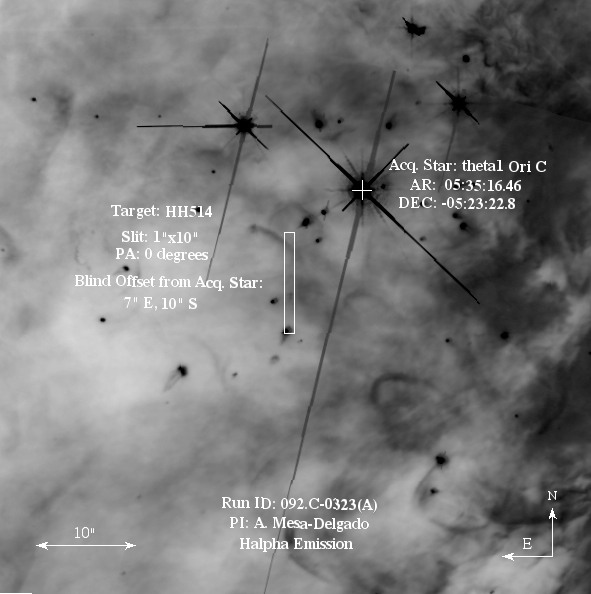
\includegraphics[width=\textwidth]{finding_HH514_halpha.jpg}
\caption{Aqui va imagen de HST}
\label{fig:hst}
\end{figure*} 



\section{Observations and data reduction}
\label{sec:data}

During the nights of October 29 and 30 of 2013, the observations were taken under clear conditions using the instrument UVES in the UT2 telescope of the Very Large Telescope (VLT). The central coordinates of the 10 arcsec slit are: RA(J2000)=05$^h$35$^m$16$^s$.95, DEC(J2000)=$-$05$^{\circ}$23$'$33.72$''$ oriented along the north-south spatial axis as is shown in Fig.~\ref{fig:hst}. The slit aperture provides an effective spectral resolution of $\lambda/\Delta \lambda \approx 6.5 \text{ km s}^{-1}$ in the spectral range between 3100-10400\AA. Analogously to the observations described in the articles on HH~529~II-III and HH~204 \citep[][hereinafter Paper~I and Paper~II, respectively]{mendez2021,mendez2021-2}, 3 exposures of 150s of the star GD71 \citep{Moehler14a, Moehler14b} were taken during the same night under similar conditions to achieve the correct flux calibration of the science data. The configuration of the instrument and the data reduction procedure are described in Paper~I while the main observational settings are shown in Table~\ref{tab:obs_set}. We define three spatial cuts along the observed slit as it is shown in Fig.~\ref{fig:cuts}, covering the main high-velocity features located around $\sim 150\text{ km s}^{-1}$ in the heliocentric velocity scale. We name the southernmost component (within cut~1) as HH~514~I while the one located in the central cut is HH~514~II. The nebular emission of cut~1 also contains the emission of the proplyd 170-337. The complete analysis of the physical conditions and chemical composition of this proplyd will be the subject of M\'endez-Delgado et al. (in prep). In this work we will only mention some results on the abundance of S in 170-337, which is of interest for our analysis of HH~514~I-II. As is shown in panel (b) of Fig.~\ref{fig:cuts}, there are several outflows of smaller velocity than HH~514 emitting mainly in the lines of highly ionized ions such as [O\thinspace III] or [Ne\thinspace III]. Unfortunately, their emission is very weak in most lines, so the determination of the physical conditions and chemical abundances of these gas components would not be reliable with the present data. To increase the contrast of the HH~514~I-II emission, which is weak compared to the main nebular emission, we subtract Cut~3 --which contains only nebular emission-- from Cut~1 and Cut~2, rescaling its emission by the number of pixels. In addition to increasing the contrast of the HH~514~I-II emission, this has the secondary benefits of eliminating sky and ghost emissions in the high-velocity spectra. We estimate the flux of the emission lines, their FWHM and their wavelength position by gaussian fittings using the SPLOT task of IRAF\footnote{IRAF is distributed by National Optical Astronomy Observatory, which is operated by Association of Universities for Research in Astronomy, under cooperative agreement with the National Science Foundation} \citep{Tody93} as is described in detail in Paper~I. We achieve the reddening correction by using the same procedure described in Paper~I and Paper~II. The values of $\text{c}(\text{H}\beta)$, are presented in Table~\ref{tab:c_extin}. 

\begin{table}
\caption{Main parameters of UVES spectroscopic observations.}
\label{tab:obs_set}
%\begin{adjustbox}{width=\columnwidth}
\begin{tabular}{ccccc}
\hline
Date & $\Delta \lambda$& Exp. time  &Seeing &Airmass\\
 & (\AA) &  (s) & (arcsec)&\\
\hline
2013-10-30 & 3100-3885 & 5, 3$\times$180 &0.92&1.11\\
2013-10-30 & 3750-4995 & 5, 3$\times$600 & 0.87 & 1.15\\
2013-10-30 & 4785-6805 & 5, 3$\times$180 &0.92&1.11\\
2013-10-30 & 6700-10420 & 5, 3$\times$600 & 0.87 & 1.15\\
\hline
\end{tabular}
%\end{adjustbox}
\end{table}


\begin{figure*}
  \begin{subfigure}{6cm}
    \centering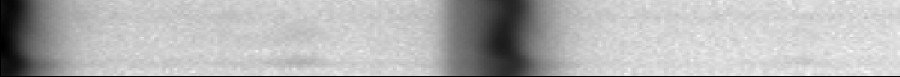
\includegraphics[height=2cm,width=\columnwidth]{2D_3729.pdf}
    \caption{[O\thinspace II] $\lambda 3729$.}
  \end{subfigure}
  \begin{subfigure}{6cm}
    \centering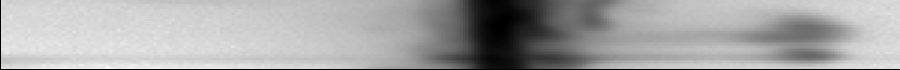
\includegraphics[height=2cm,width=\columnwidth]{2D_4959.pdf}
    \caption{[O\thinspace III] $\lambda 4959$.}
  \end{subfigure}
 
  \begin{subfigure}{6cm}
    \centering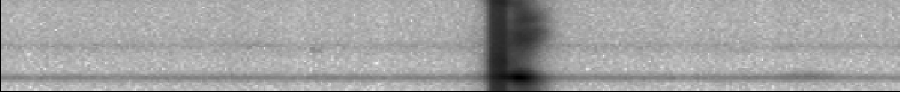
\includegraphics[height=2cm , width=\columnwidth]{2D_6300.pdf}
    \caption{[O\thinspace I] $\lambda 6300$.}
  \end{subfigure}
  \begin{subfigure}{6cm}
    \centering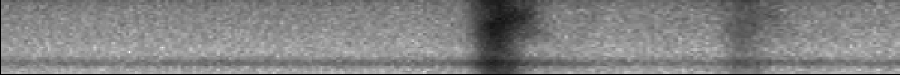
\includegraphics[height=2cm , width=\columnwidth]{2D_4649.pdf}
    \caption{O\thinspace II $\lambda 4649$.}
  \end{subfigure}
\begin{subfigure}{12.0cm}
\centering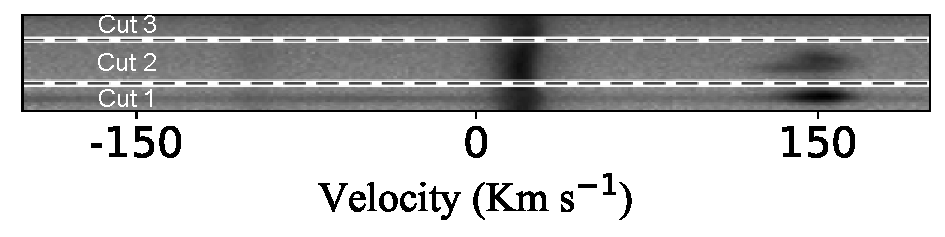
\includegraphics[height=4cm, width=\columnwidth]{2D_4658_cuts_named.pdf}
\caption{[Fe\thinspace III] $\lambda 4658$.} 
\end{subfigure}

\caption{\textit{Upper panels:} Sample of representative lines in the bi-dimensional spectrum. The Y axis corresponds to the spatial direction (up north, down south, see Fig.~\ref{fig:hst} for the spatial location of the slit) while the X axis is the spectral axis. All figures are centred at $\lambda_0$, the rest-frame reference wavelength of each line. \textit{Bottom panel:} Emission of the [Fe\thinspace III] $\lambda 4658.17$ line as well as the limits and extension of the different spatial cuts selected to analyse each velocity component. Cut 1 is at the bottom, which corresponds to the southernmost one. The spatial coverage is 2.71 arcsec, 4.18 arcsec and 2.46 arcsec for cuts 1, 2 and 3, respectively. The velocity scale is heliocentric.}
\label{fig:cuts}
\end{figure*}




\begin{table}
\caption{Reddening coefficients for each component.}
\label{tab:c_extin}
%\begin{adjustbox}{width=\columnwidth}
\begin{tabular}{lccccc}
\hline
 & \multicolumn{2}{c}{$\text{c}(\text{H}\beta)$} \\
  & Nebular & High velocity\\
\hline
Cut 1 & - & $0.78 \pm  0.03$  \\
Cut 2 & $0.85 \pm 0.03$ &$0.72 \pm 0.03$\\
Cut 3 & $0.85 \pm 0.02$&-\\
\hline
\end{tabular}
%\end{adjustbox}
\end{table}





\section{Physical Conditions}
\label{sec:physical_cond}

We use the version 1.1.13 of PyNeb \citep{Luridiana15} and the atomic data set shown in Tables 9 and 10 from Paper~II to derive the physical conditions of the different gas  components analyzed in this work. The adopted density in the nebular components is a weighted average\footnote{The weights were defined as the inverse of the square of the error associated to each density diagnostic.} of the resulting values from the CEL diagnostics
[O\thinspace II] $\lambda3726/\lambda3729$, [S\thinspace II] $\lambda6731/\lambda6716$, [Cl\thinspace III] $\lambda5538/\lambda5518$, [Fe\thinspace II] $\lambda9268/\lambda9052$, [Fe\thinspace III] $\lambda4658/\lambda4702$ and [Ar\thinspace IV]  $\lambda4740/\lambda4711$.  We follow the maximum-likelihood procedure described in Sec.~4.2 of Paper~I to derive the physical conditions based on the [Fe\thinspace III] $\lambda \lambda $ 4658, 4702, 4734, 4881, 5011 and 5271 lines. As it was commented in Paper~I, with the adopted atomic data, [Fe\thinspace III] diagnostics are not very sensitive to density at smaller values than $10^{3} \text{ cm}^{-3}$, thus if a considerable part of the observed ionized gas has similar or lower densities than this value (as it is expected along the line of sight in the nebular components), the resulting $n_{\rm e}$ may be biased to the higher densities integrated in the line of sight. $n_{\rm e}(\text{O\thinspace II})$ was derived with the available RLs of multiplet 1 and the results are highly consistent with the adopted average density.

In the plasma diagnostic plot of HH~514~I in Fig.~\ref{fig:plasma}, the curve of the temperature diagnostic  [N\thinspace II] $\lambda5755/\lambda6584$ suggest either an extremely high density (greater than 10$^5$ cm$^{-3}$) or an extremely high temperature (higher than 10$^{5}$ K at smaller densities than 10$^{4}$ cm$^{-3}$). The [Fe\thinspace III] $\lambda4658/\lambda4702$, [S\thinspace II] $\lambda$4069/$\lambda$4076 and [O\thinspace II] $\lambda$7319+20/$\lambda$7330+31 density diagnostics confirms the first case. In HH~514~I-II we estimate the convergence of $n_{\rm e}-T_{\rm e}$ by using the [Fe\thinspace III] $\lambda \lambda$ 4658, 4702, 4734, 4881, 5011, 5271 CELs. The resulting density of In HH~514~I is $10^{5.37} \text{ cm}^{-3}$, one of the highest densities estimated for a photoionized region. 

In the case of HH~514~II, the convergence shows a higher dispersion in $n_{\rm e}-T_{\rm e}$ which seems to be due to the mixture of two or more gas components with similar velocities and notably different physical and/or ionization conditions. As is shown in Fig.~\ref{fig:spatial_dis}, the spatial distribution of the emission at $\sim 150 \text{ km s}^{-1}$ from the [Fe\thinspace III] $\lambda 4658$ line is double-peaked in HH~514~II, which shows that at least two different gas components moving at a similar velocity are integrated in HH~514~II. However, the separation into two spatial components results in a very low signal-to-noise spectra. Thus, the physical conditions and chemical abundances derived in HH~514~II are expected to have greater uncertainties than those from HH~514~I.

Based on the adopted density in each component, we estimate $T_{\rm e}$ through various diagnostics shown in Table~\ref{tab:pc}. In the nebular components, we define $T_{\rm e} \text{ (low)}$ as the weighted average of $T_{\rm e} (\text{[N\thinspace II]})$, $T_{\rm e} (\text{[O\thinspace II]})$ and $T_{\rm e} (\text{[S\thinspace II]})$ while $T_{\rm e} \text{ (high)}$ is the weighted average of $T_{\rm e} (\text{[O\thinspace III]})$, $T_{\rm e} (\text{[S\thinspace III]})$ and $T_{\rm e} (\text{[Ar\thinspace III]})$. It is noticeable that, despite of the extremely high density of HH~514~I-II, the temperature is consistent with the expected values in the photoionization equilibrium. There it seems to be a slightly underprediction of $T_{\rm e}(\text{[S\thinspace III]})$, which would be expected to be equal to or greater than $T_{\rm e}(\text{[O\thinspace III]})$ due to temperature stratification \footnote{Photons with energies close to the photoionization threshold of the elements are more easily absorbed since the photoionization absorption cross section values decrease as the energy of the photon increases \citep{osterbrock06}. This causes the less energetic photons (with energies greater than the ionization threshold) to be absorbed first than the more energetic ones, which generally implies that the areas with a lower degree of ionization of the nebula are hotter. Since the ionization potential of S$^{2+}$ is lower than that of O$^{2+}$, we would expect, at first approximation, $T_{\rm e}(\text{[S\thinspace III]})\geq T_{\rm e}(\text{[O\thinspace III]})$.}. This behaviour of $T_{\rm e}(\text{[S\thinspace III]})$ may have a common origin with an apparent overabundance of S$^{2+}$ in HH~514~I-II. This is gonna be discussed in Sec.~\ref{sec:under_TS3}. In both HH~514~I and HH~514~II, the estimation of $T_{\rm e} \text{ (low)}$ is quite uncertain, given the low critical density of the diagnoses observed in this ionization zone and the high density of these objects. Due to this, and considering the similarity between $T_{\rm e}(\text{[O\thinspace III]})$ in both velocity components, we will adopt the same value of $T_{\rm e} \text{ (low)}$ in HH~514~I and HH~514~II, using the estimated value in HH~514~I, the spectrum with the best signal to noise ratio.


\begin{figure}
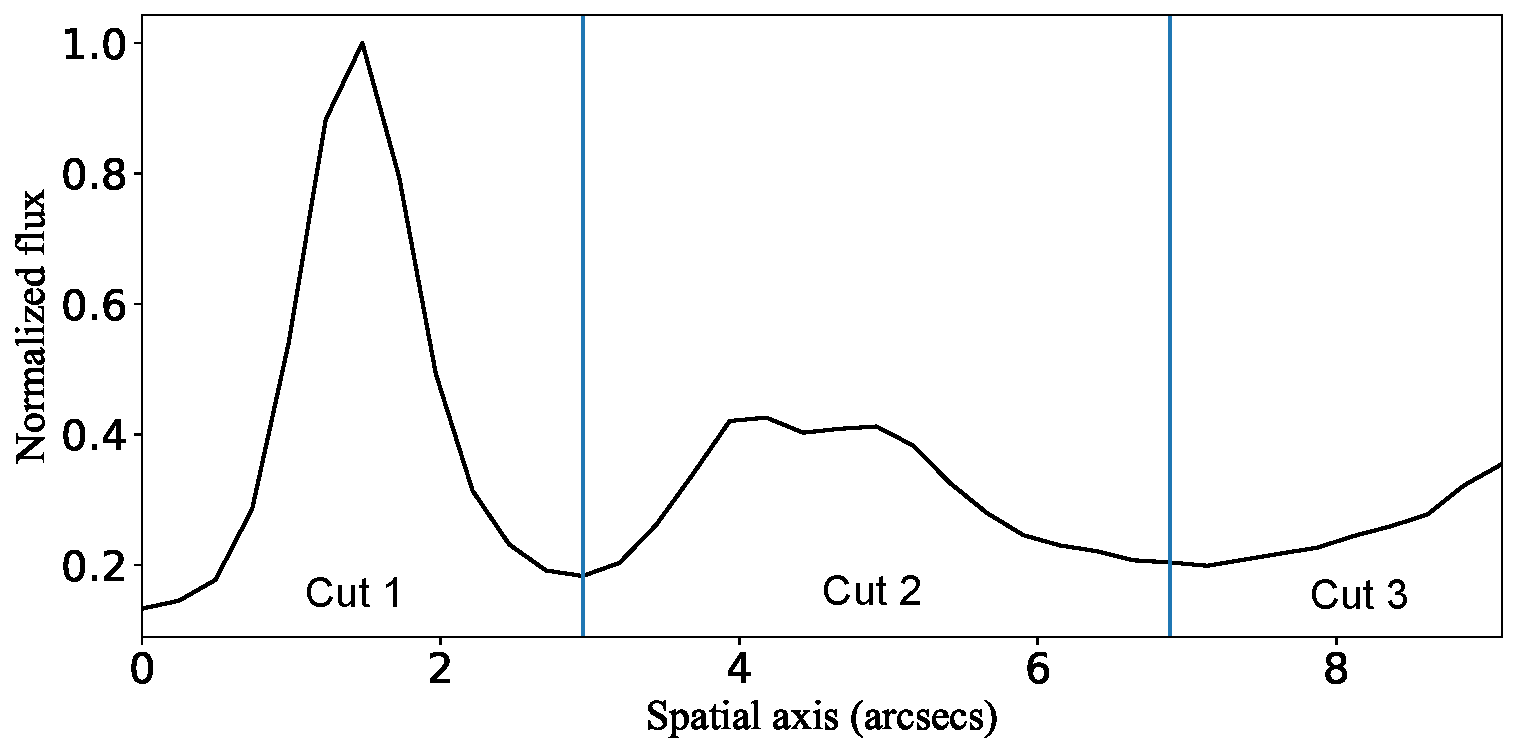
\includegraphics[width=\columnwidth]{brillo_4658_HH514.pdf}
\caption{Emission distribution in a $\sim 45 \text{ km s}^{-1}$ window along the spatial axis centred around $\sim 150 \text{ km s}^{-1}$ from the [Fe\thinspace III] $\lambda 4658$ line.}
\label{fig:spatial_dis}
\end{figure}




\begin{table*}
\centering
\caption{Physical conditions determined from  several diagnostics.}
\label{tab:pc}
%\begin{adjustbox}{width=\textwidth}
\begin{tabular}{ccccc}
\hline 
 & \multicolumn{1}{c}{Cut 1} & \multicolumn{2}{c}{Cut 2} & \multicolumn{1}{c}{Cut 3} \\
Diagnostic & HH514-I & Nebula & HH514-II  & Nebula\\
\hline
& \multicolumn{4}{c}{$n_e$(cm$^{\text{-}3}$)}\\


[O\thinspace II] $\lambda$3726/$\lambda$3729 &  - &$5980^{+1160} _{-870}$&  - & $5610^{+960} _{-800}$\\

[O\thinspace II] $\lambda$7319+20/$\lambda$7330+31 &  263030: & - & - &- \\

[S\thinspace II] $\lambda$6731/$\lambda$6716 & - & $4150^{+1810} _{-1230}$&  -& $4240^{+1400} _{-1030}$\\

[S\thinspace II] $\lambda$4069/$\lambda$4076 & 218780: & - &-&-\\

[Cl\thinspace III] $\lambda$5538/$\lambda$5518 & - & $7640^{+970} _{-1020}$&  -& $7620^{+1070} _{-960}$\\

[Fe\thinspace II] $\lambda$9268/$\lambda$9052 & >75860 & $4500^{+9740} _{-3590}$ &  -& $3540^{+9190} _{-2760}$ \\

[Fe\thinspace III] $\lambda$4658/$\lambda$4702 & 234420: & $8490^{+2490} _{-2350}$& 57020: & $6430^{+2810} _{-2080}$\\

[Ar\thinspace IV]  $\lambda$4740/$\lambda$4711 & - &$6730^{+660} _{-690}$& - & $4800^{+570} _{-690}$\\


O\thinspace II$^{*}$  & - &$5640 \pm 510$&-&$4960 \pm 650$ \\

[Fe\thinspace III]$^{*}$ & $231820 \pm 12120$ & $8600 \pm 810$ & $74240 \pm 14220$& $7540\pm 1020$\\ 


\textbf{Adopted} &  \boldmath${231820 \pm 12120}$ &  \boldmath${6690 \pm 940}$&  \boldmath${74240 \pm 14220}$&  \boldmath${5490 \pm 1120 }$\\

 & \multicolumn{4}{c}{$T_e$ (K)}\\

T$\left(\mbox{He}\thinspace \mbox{I} \right)$ & $8710:$&$7790 ^{+570} _{-480}$ & $6010:$&$7570 ^{+490} _{-550}$\\

[N\thinspace II] $\lambda$5755/$\lambda$6584  & $12860^{+1240} _{-1170}$& $9750^{+230} _{-220}$&- &$9880^{+230} _{-250}$\\

[O\thinspace II] $\lambda \lambda$ 3726+29/$\lambda \lambda$7319+20+30+31 & $9180^{+1500} _{-630}$& $9500^{+740} _{-610}$& $7830^{+1430} _{-810}$&$10980^{+1040} _{-1320}$\\

[S\thinspace II] $\lambda \lambda$4069+76/$\lambda \lambda$ 6716+31& $20010^{+45030} _{-9150}$& $9410^{+950} _{-1220}$&-&$10090^{+2180} _{-1400}$\\

[O\thinspace III] $\lambda$4363/$\lambda \lambda$4959+5007& $8880^{+250} _{-210}$& $8490^{+90} _{-100}$ & $9330^{+260} _{-230}$& $8400^{+80} _{-70}$\\

[S\thinspace III] $\lambda$6312/$\lambda \lambda$9069+9531 & $8420^{+310} _{-400}$& $8630^{+330} _{-340}$& $8230^{+430} _{-560}$ & $8820^{+330} _{-310}$\\

[Ar\thinspace III]  $\lambda$5192/$\lambda$7136  & - & $8070^{+190} _{-160}$&-&$8320^{+230} _{-190}$\\

[Fe\thinspace III]$^{*}$ & $6840 \pm 1640$ & $8960 \pm 850$ & $8180 \pm 1410$& $7850 \pm 830$\\

\textbf{\boldmath${T_e}$ (low) Adopted} & \boldmath${11370 \pm 1820}$ & \boldmath${9530 \pm 100}$& \boldmath${11370 \pm 1820}$ & \boldmath${9920 \pm 200}$\\


\textbf{\boldmath${T_e}$ (high) Adopted} & \boldmath${8880 \pm 250}$ & \boldmath${8430 \pm 150}$ & \boldmath${9330 \pm 260}$ & \boldmath${8410 \pm 100}$\\

\hline
\end{tabular}
%\end{adjustbox}
\end{table*}

%RMS6742=9.787e-17
%upperlimit-1sigma=3.435577660528658e-17
%upperlimit-3sigma=1.0306732981585972e-16
%6742HB-1sigma=0.080953722395563323
%6742HB-3sigma=0.24286116718668996
%upper-lim-1sigma=6.99
%upper-lim-3sigma=7.47


\section{Ionic and Total Abundances}
\label{sec:ionic_total_abundances}

We derive the ionic abundances of Ni$^{+}$, Fe$^{+}$, Ca$^{+}$, O$^{+}$, N$^{+}$, S$^{+}$, Cl$^{+}$ based on CELs, associating $T_{\rm e} \text{ (low)}$ to these ions. In these spectra, we derive the abundances of S$^{2+}$ and Cl$^{2+}$ using $T_{\rm e} \text{ ([S\thinspace III])}$ and the ionic abundances of Ar$^{2+}$, Cl$^{3+}$, Ar$^{3+}$, Fe$^{3+}$, O$^{2+}$ and Ne$^{2+}$ based on $T_{\rm e} \text{ (high)}$. In HH~514~I-II, we derive Fe$^{2+}$, Ni$^{2+}$ using $T_{\rm e} \text{ (high)}$ while in the nebular component we use $T_{\rm e} \text{ (low)}$, since for the high velocity components, $T_{\rm e} \text{ ([Fe\thinspace III])}$ suggest a better association of Fe$^{2+}$ with the physical conditions of the gas of high degree of ionization. Since in Paper~II we showed that the ionic abundances of Ni and Fe are correlated, showing similar depletion and ionization patterns, the same temperature was used to estimate the abundance of Ni$^{2+}$. In the case of Ca$^+$, caution must be taken due to the possible coexistence of Ca$^+$ in the neutral hydrogen volume, due to its low ionization potential.



¿la fluorescencia en Ni+?

%na/nb=1/r**2_a/1/r**2_b= r**2_b/r**2_a= 12.61**2/63.98**2= 0.038845588175657815

nb=55860






In the nebular spectra we estimate the abundances of He$^{+}$, O$^{+}$, C$^{2+}$, O$^{2+}$ and Ne$^{2+}$ from RLs following the same procedure described in Paper~I. In the case of HH~514~I and HH~514~II, we only determine the abundance of He$^{+}$ from RLs. In this case, the adopted He$^{+}$ abundance is an average from the resulting values based on the available He\thinspace I singlet lines and triplet lines less affected by self absorption effects (See Table D14 from Paper~I). The results are shown in Table~\ref{tab:rls_abundances}. 

\begin{table*}
\centering
\caption{Chemical abundances based on CEL's.}
\label{tab:cels_abundances}
%\begin{adjustbox}{width=\textwidth}
\begin{tabular}{ccccccccccccc}
\hline
 & \multicolumn{1}{c}{Cut 1} & \multicolumn{2}{c}{Cut 2} & \multicolumn{1}{c}{Cut 3} & \\
Ion &  HH~514~I & Nebula & HH~514~II  & Nebula \\
\hline

O$^{+}$ & $7.93^{+0.51} _{-0.18}$ & $7.81 \pm 0.03 $&$7.40^{+0.49} _{-0.19}$ & $7.69 \pm 0.05 $\\ 

O$^{2+}$ & $8.30^{+0.05} _{-0.04}$& $8.37 \pm 0.03$& $8.45^{+0.05} _{-0.04}$ &$8.38 \pm 0.02 $\\

N$^{+}$  & $6.88^{+0.28} _{-0.13}$ &$6.89 \pm 0.02 $  & $6.23^{+0.27} _{-0.14}$& $6.84 \pm 0.03 $\\

Ne$^{2+}$ & $7.56^{+0.06} _{-0.05}$& $7.84^{+0.04} _{-0.03}$ & $7.79^{+0.06} _{-0.05}$&$7.82^{+0.03} _{-0.02}$\\

S$^{+}$ & $6.11^{+0.23} _{-0.12}$ & $5.50 \pm 0.04 $& $5.34^{+0.26} _{-0.14}$&$5.45 \pm 0.05 $\\

S$^{2+}$ & $7.39^{+0.07} _{-0.06}$ &$6.86^{+0.05} _{-0.04}$ & $7.35^{+0.09} _{-0.07}$&$6.84^{+0.05} _{-0.04}$\\

Cl$^{+}$ & - &$3.63 \pm 0.04 $&- &$3.60 \pm 0.04 $\\

Cl$^{2+}$ &- &$4.98^{+0.06} _{-0.05}$&- &$4.99^{+0.06} _{-0.05}$\\

Cl$^{3+}$ & - &$3.79 \pm 0.03 $&- &$3.92 \pm 0.03 $\\

Ar$^{2+}$ & $6.29 \pm 0.04 $& $6.31 \pm 0.03 $& $6.19 \pm 0.04 $&$6.31 \pm 0.02 $\\

Ar$^{3+}$ & - &$5.09^{+0.04} _{-0.03}$& -&$5.15^{+0.03} _{-0.02}$\\

Fe$^{+}$ & $6.14 \pm 0.05$ & $4.39 \pm 0.05$ & - &$4.32 \pm 0.02$\\ 

Fe$^{2+}$ & $7.14 \pm 0.02$ & $5.28 \pm 0.01$& $6.83 \pm 0.04$&$5.17 \pm 0.02$\\

Fe$^{3+}$ & < 6.99 &$5.62^{+0.10} _{-0.08}$& -&$5.78 \pm 0.12 $\\

Ni$^{+}$ & $4.94^{+0.15} _{-0.09}$ & - &-&-\\

Ni$^{2+}$ &$5.84^{+0.07} _{-0.06}$ & $4.32 \pm 0.03 $ &$5.62^{+0.08} _{-0.07}$&$4.25 \pm 0.04 $\\

Ca$^{+}$ & $3.71^{+0.20} _{-0.12}$ &- &-&-\\

\hline
\end{tabular}
%\end{adjustbox}
\end{table*}








%Fe3: se usan las lineas mas intensas de cada nivel superior de origen para promediar.






\begin{table*}
\centering
\caption{Chemical abundances based on RL's}
\label{tab:rls_abundances}
%\begin{adjustbox}{width=\textwidth}
\begin{tabular}{ccccccccccccc}
\hline
 & \multicolumn{1}{c}{Cut 1} & \multicolumn{2}{c}{Cut 2} & \multicolumn{1}{c}{Cut 3} & \\
Ion &  HH~514~I & Nebula & HH~514~II  & Nebula \\
\hline

He$^{+}$  &$10.95 \pm 0.04$  & $10.92 \pm 0.02$& $10.96 \pm 0.02$&$10.92 \pm 0.02$\\

O$^{+}$ & - & $8.17^{+0.04} _{-0.03}$& -& $8.19 \pm 0.05 $ \\

O$^{2+}$ & - & $8.61 \pm 0.05$ & - & $8.63 \pm 0.05$  \\

C$^{2+}$  & -& $8.37 \pm 0.01 $ &-&  $8.37 \pm 0.01$ \\

Ne$^{2+}$ & -&$8.04 \pm 0.06 $&-& $8.10 \pm 0.08 $ \\
 
\hline
\end{tabular}
%\end{adjustbox}
\end{table*}

To estimate the total abundances of some elements, we use the Ionization Correction Factors (ICFs) shown in Table~10 from Paper~I. An exceptional case is the Ni abundances,  estimated as $\text{Fe/Ni}=\text{Fe}^{2+}/\text{Ni}^{2+}$ based on their similar depletion and ionization patterns \citep[][]{mendez2021-2}. In the nebular spectra, the calculation of the total abundances of O, Cl, Ar and Fe did not require ICF and were estimated from the sum of their ionic abundances. On the other hand, in the high-velocity components, we do not use any ICF for the estimation of the total abundance of O and He. The results are shown in Table~\ref{tab:total_abundances_cels} and Table~\ref{tab:total_abundances_rls}.


\begin{table*}
\centering
\caption{Total abundances based on CELs.  The units are logarithmic with $n(\text{H})=12$.}
\label{tab:total_abundances_cels}
%\begin{adjustbox}{width=\textwidth}
\begin{tabular}{ccccccccccccc}
\hline
 & \multicolumn{1}{c}{Cut 1} & \multicolumn{2}{c}{Cut 2} & \multicolumn{1}{c}{Cut 3} & \\
Ion &  HH~514~I & Nebula & HH~514~II  & Nebula \\
\hline

O  & $8.44 \pm 0.03$& $8.46 \pm 0.03$&$8.73 \pm 0.10$&$8.46 \pm 0.02$\\

N  & $7.58 ^{+0.07} _{-0.06}$& $7.56 ^{+0.05} _{-0.04}$ & $7.83 ^{+0.31} _{-0.15}$&$7.61 ^{+0.05} _{-0.04}$\\ 

Ne & $7.69 \pm 0.05$ & $7.93 \pm 0.04$ & $8.02 \pm 0.10$&$7.89 \pm 0.03$\\ 

S  & $7.46 \pm 0.04$ & $6.98 \pm 0.05$ & $7.74 ^{+0.11} _{-0.08}$&$6.99 \pm 0.04$\\

Cl & - & $5.01 \pm 0.05$ & - & $5.04 \pm 0.04$\\

Ar & $6.31 \pm 0.03$ & $6.33 \pm 0.03$ & $6.46 ^{+0.15} _{-0.10}$&$6.33 \pm 0.02$\\

Fe & 7.54--7.70 & $5.76 \pm 0.07$ & 7.60--8.10&$5.87 \pm 0.10$\\

Ni & 6.16--6.32 & $4.82 \pm 0.08$ &6.38--6.88& $4.95 \pm 0.11$ \\


\hline
\end{tabular}
%\end{adjustbox}
\begin{description}
\item $^*$ asd. \\
\end{description}
\end{table*}




\begin{table*}
\centering
\caption{Total abundances based on RLs.  The units are logarithmic with $n(\text{H})=12$.}
\label{tab:total_abundances_rls}
%\begin{adjustbox}{width=\textwidth}
\begin{tabular}{ccccccccccccc}
\hline
 & \multicolumn{1}{c}{Cut 1} & \multicolumn{2}{c}{Cut 2} & \multicolumn{1}{c}{Cut 3} & \\
Ion &  HH~514~I & Nebula & HH~514~II  & Nebula \\
\hline

He  & $10.94 \pm 0.02$ & $10.95 \pm 0.02$ & $10.96 \pm 0.03$&$10.95 \pm 0.02$\\

O  &  - & $8.74 \pm 0.04$ &-&$8.76 \pm 0.04$\\ 

C & - &$8.50 \pm 0.02$ &-&$8.50 \pm 0.02$\\ 

Ne  & - &$8.18 \pm 0.06$&-&$8.24 \pm 0.08$\\

\hline
\end{tabular}
%\end{adjustbox}
\begin{description}
\item $^*$ asd. \\
\end{description}
\end{table*}


\section{On the anomalous [S\thinspace III] emission in HH~514}
\label{sec:under_TS3}

Plasma diagnostics from Fig.~\ref{fig:plasma} for HH~514~I and HH~514~II show that $T_{\rm e} \text{ ([S\thinspace III])}$<$T_{\rm e} \text{ ([O\thinspace III])}$. In the case of HH~514~I the difference is small and falls within error bars. However, in the case of HH~514~II the plasma curves do not intersect. This result is complex to interpret because it goes in the opposite direction to the usual temperature stratification observed in H~II regions and simple photoionization models fail to reproduce the observed result \citep[][]{Binette2012}.

In the case of the S$^{2+}$ abundances, they were derived from [S\thinspace III] I($\lambda 9531$) since [S\thinspace III] I($\lambda 9069$) is slightly affected by a telluric absorption band. 









\section{The apparent sulphur overabundance in HH~514~I-II}
\label{sec:over_sulphur}












\section{Discussion}


\subsection{The nebular spectra }
\label{subsec:disc_neb_comp}

The spectra of the nebular components of cut~2 and cut~3 are dominated by the emission of the Orion Nebula in an area very close the Trapezium, around $\sim 10 \text{ arcsecs}$ from $\theta^{1} \text{ Ori C}$, its main ionization source, although the emission of gas moving at slightly different velocities is also contributing to the spectra (see Fig.~\ref{fig:cuts}). These gas components may be originated in small shocks between the nebular gas and material ejected from young stars and proplyds, visible in great numbers in the area. However, their global influence is rather negligible since their emission is very weak compared to the nebular one. The physical conditions and ionic abundances of the nebular components in this work are rather similar to those found in Paper~I, despite of their different distances from the main ionization source (the observed area in Paper~I is around $\sim 35$ arcsec from $\theta^{1} \text{ Ori C}$).% However, there are some exceptions that we will discuss below. 

By comparing the ionic abundances derived with CELs with those estimated with RLs of O$^{+}$, O$^{2+}$, Ne$^{2+}$ we can directly estimate the Abundance Discrepancy Factor (ADF) of each element. In the case of the ionic abundance of C$^{2+}$, we adopt the abundance based on CELs derived by \citet{walter92} in their position 5, the closest to our observed area in order to estimate an ADF(C$^{2+}$). The results are shown in Table\ref{tab:ADF} together with a comparison of results with data of similar quality.


\begin{table*}
\centering
\caption{The ADF in the Orion Nebula.}
\label{tab:ADF}
%\begin{adjustbox}{width=\textwidth}
\begin{tabular}{ccccccccccccc}
\hline
Distance to $\theta^{1} \text{ Ori C}$  (arcsecs)&  ADF(O$^{+}$) & ADF(O$^{2+}$) & ADF(Ne$^{2+}$) & ADF(C$^{2+}$)$^{*}$ & Reference\\
\hline
12.61 & $0.41\pm 0.08$ & $0.24 \pm 0.08$ & $0.20 \pm 0.10$& $0.54 \pm 0.01$ & This work\\
29.44 & $0.39 \pm 0.28$& $0.14 \pm 0.02$ & $0.26\pm 0.14$ & $0.43\pm 0.14$ &\citet{Esteban04}\\
34.96 & $0.42 \pm 0.12$ &$0.17 \pm 0.05$ & $0.37\pm 0.04$ &$0.52 \pm 0.03$ &\citet{mendez2021}\\
75.94 & $0.01\pm 0.17$ & $0.11\pm 0.04$ & - &$0.45 \pm 0.07$ & \citet{mesadelgado09}\\
150.40 & - & $0.36 \pm 0.05$&-& $1.09\pm 0.01$& \citet{mendez2021-2}\\
\hline
\end{tabular}
%\end{adjustbox}
\begin{description}
\item $^*$ We adopt the C$^{2+}$ abundances based on CELs from \citet{walter92}. \\
\end{description}
\end{table*}



\begin{table*}
\centering
\caption{[SIII] values corrected from telluric abs}
\label{tab:tellabs}
%\begin{adjustbox}{width=\textwidth}
\begin{tabular}{ccccccccccccc}
\hline
Object &   \multicolumn{2}{c}{$\lambda 9069$} & \multicolumn{2}{c}{$\lambda 9531$} & Reference\\
 & Old & New  & Old & New & \\
\hline

Orion Nebula Cut 1 & $19.713 \pm 0.985$ & $32.148\pm 1.929$& $82.845 \pm 4.971$ & $84.653 \pm 5.926$ & \multirow{4}{*}{\citet{mendez2021}}\\

Orion Nebula Cut 2 & $20.807 \pm 1.248$ &  $32.543 \pm 2.278$& $91.130\pm 5.468$&$91.438 \pm 6.401 $\\

Orion Nebula Cut 3 & $21.792\pm 1.308$ & $31.778\pm 1.907$& $91.118\pm 6.378$&$91.355 \pm 6.395$\\

Orion Nebula Cut 4 &$22.765 \pm 1.366$ & $ 34.075 \pm 2.385$ & $82.527\pm 4.952$ & $85.145\pm5.960$\\


Orion Nebula + NIL Cut 1 & $25.379\pm 1.015$ & $28.562\pm 1.428$ & $ 69.320 \pm 2.773$ & $69.330 \pm 3.466$ & \multirow{2}{*}{\citet{mendez2021-2}}\\

Orion Nebula Cut 2 & $24.746\pm 1.237$ & $30.686\pm 1.841$ & $74.642\pm 4.478$ & $74.643\pm 5.225$ \\

HH529II & \multicolumn{2}{c}{$40.116 \pm 2.407$} &  \multicolumn{2}{c}{$98.517 \pm 6.896$}&\multirow{2}{*}{\citet{mendez2021}}\\

HH529III & \multicolumn{2}{c}{$41.104 \pm 3.288$} &  \multicolumn{2}{c}{$100.396 \pm 9.036$}&\\

HH204 & \multicolumn{2}{c}{$36.535 \pm 1.461$} & \multicolumn{2}{c}{$87.222\pm 3.489$}\\

NIL & $26.541\pm 2.919$ & $20.695\pm2.483$& $ 60.608\pm 6.667$& $55.487\pm 6.658$& \citet{mendez2021-2}\\

--------
NEBULAR cut2 &$23.865\pm 1.432$& $31.843\pm2.229$ & $85.893\pm 6.013$ & $85.910 \pm  6.872$ \\ 

NEBULAR cut3 &$23.676\pm 1.420$ & $31.122\pm 2.179$ & $85.362\pm 5.122$ & $81.153\pm 5.680$\\ 


HH514I & $72.951\pm 5.836$ &$74.610\pm6.715$ & $194.920\pm 15.594$&$194.289 \pm 17.486$\\ 

HH514II & $82.483\pm 7.424$ &$87.074\pm 8.707$&$217.667\pm21.767$&$ 220.679\pm24.274 $\\ 


\hline
\end{tabular}
%\end{adjustbox}
\end{table*}



Para sustraer  [SIII] del blend con H14, se usa la medida de H15 y el cociente teorico de H14/H15. Esto es asi viendo la figura 5 de \citet{mesadelgado09} donde las lineas de Balmer de alto n se alejan de lo predicho por el Caso B del atomo de hidrogeno. H14 y H15 tienen un comportamiento similar, y aunque H14/HB y H15/HB esten mas intensas de lo predicho, H14/H15 si estan mas o menos bien predichas por el caso B 

mmm mejor no. mejor solo ver 3721/6312 en las regiones donde se separan bien con un deblend y donde solo hay una componente cinematica de emision. la FWHM del 3721 debe ser consistente con la de 6312



No se incluye 30 doradus porque esos errores del 1.2 porciento no se los creo. Es evidente que hay una banda telurica en 9531, considerando su velocidad radial
\begin{table*}
\centering
\caption{}
\label{tab:atomic_data_test}
%\begin{adjustbox}{width=\textwidth}
\begin{tabular}{ccccccccccccc}
\hline
Reference & 3722/6312 & 9531/9069 & 9531/8829 &9069/8829 \\
\hline
---Orion Nebula---\\

\citet{Esteban04} & - & $2.39 \pm 0.51$ & $5576.37 \pm 1326.47$ & $2313.96 \pm 539.11$\\

\citet{mesadelgado09} & - & $2.32 \pm 0.19$ & - & - \\

\citet{mendez2021} Cut 1 & $0.60 \pm 0.03$ & $2.65 \pm 0.24$ & $8414.88 \pm 1221.90$ & $3204.57 \pm 455.63$\\

\citet{mendez2021} Cut 2 & - &$2.84 \pm 0.27$ & $7663.46 \pm 893.46$& $2729.17 \pm 312.05$\\

\citet{mendez2021} Cut 3 & - &$2.88 \pm 0.26$&$8259.73 \pm 1096.90$&$2875.21 \pm 365.38$\\

\citet{mendez2021} Cut 4 & - &$2.50 \pm 0.24$&$7673.32 \pm 1283.67$ & $3068.76 \pm 519.54$ \\

 
\citet{mendez2021-2} Cut 1 + NIL & - & $2.43 \pm 0.18$ &$5830.90 \pm 672.89$&$2397.19 \pm 272.37$ \\

\citet{mendez2021-2} Cut 2 & - & $2.44 \pm 0.22$ & $6752.15 \pm 1162.68$& $2789.65 \pm 474.00$ \\

\citet{mendez2021-2} NIL & - &$2.65 \pm 0.46$ &-&- \\

This work Cut 2 & $0.64 \pm 0.02$ & $2.69 \pm 0.28$ & $7771.60 \pm 1077.27$ & $2892.90 \pm 392.05$\\


This work Cut 3 & - & $2.60 \pm 0.27$ & $7388.21 \pm 972.74$ & $2828.85 \pm 372.08$\\

--HHs--\\

\citet{mesadelgado09} HH202S & - & $2.54 \pm 0.22$ & -&-\\

\citet{mendez2021} HH529II &-&$2.46 \pm 0.22$&$7462.41 \pm 1822.99$&$3070.78 \pm 731.04$\\

\citet{mendez2021} HH529III &-&$2.45 \pm 0.29$ & - & -\\


\citet{mendez2021-2} HH204 & - & $2.39 \pm 0.14$ & $8721.53 \pm 966.81$ & $3632.17 \pm 405.38$\\

This work HH514I & - & $2.60 \pm 0.32$ &-&-\\

This work HH514II & - & $2.55 \pm 0.38$ &-&-\\



---HII---\\

\citet{garciarojas04} NGC3576 & -& - & - & $2478.77 \pm 396.99$ \\

\citet{garciarojas05} S311& - & $2.70\pm 0.21$&-&-\\

\citet{garciarojas06} M16 &-&$ 2.43\pm 0.29$&-&-\\

\citet{garciarojas06} M20 & -& $ 2.29\pm 0.20$&-&-\\

\citet{garciarojas06} NGC3603 & - & - & $5924.70 \pm 828.94$ & - \\

\citet{garciarojas07-2} M8 &-& - &- & $2742.62 \pm 680.99$  \\

\citet{garciarojas07-2} M17 &-& $2.51 \pm 0.25$ &-&-\\

\citet{Esteban13} NGC 2579 &- &$2.18 \pm 0.12$ &-&-\\


---PNs---\\

\citet{Sharpee03} IC 418 & -& 2.38 & 8798.08 & 3705.72\\


Adopted & \boldmath $0.62 \pm 0.03$ & \boldmath $2.45 \pm 0.18$& \boldmath$ 7217.60\pm 1168.83$ & \boldmath $2875.77\pm415.72$\\


---Theoretical---\\

Chianti & 0.53&2.51&8473.87&3372.62&\\
LL93-HSC95-MZ82b-KS86 &0.52& 5.52&14962.86&2710.07\\
MZ82b-HSC95-LL93  & 0.61 & 2.48 &9168.73&3697.08\\
FFTI06 &0.54& 2.47&8470.16&3430.85\\
TZS19 & 0.50 & 2.54&5504.84&2170.84\\

\hline
\end{tabular}
%\end{adjustbox}
\begin{description}
\item $^*$ We adopt the C$^{2+}$ abundances based on CELs from \citet{walter92}. \\
\end{description}
\end{table*}

Los valores promedio de 9531/9069 incluye a las regiones HII de \citet{Vital18}. Las PNs se escogieron porque fueron las mejor evaluadas por \citet{rodriguez20}.


**=9531 afectada
*=9069 afectada








\subsection{The impact of the atomic data on the S$^{2+}$ ion }
\label{subsec:atomic_data_siii}



\begin{table*}
\centering
\caption{}
\label{tab:atomic_data_tempsiii}
\begin{adjustbox}{width=\textwidth}
\begin{tabular}{ccccccccccccc}
\hline
 &  GMZ95 & TG99 & HRS12 & GRHK14 & TZS19 & Yo\\
\hline
\multicolumn{5}{c}{HH~514~I} \\
 

FFTI06  & $8370^{+420} _{-450}$ & $7980^{+400} _{-530}$ & $8410^{+350} _{-390}$ & $8420^{+310} _{-400}$ & $7900^{+480} _{-170}$ & $8840^{+500} _{-560}$ \\


\multicolumn{5}{c}{HH~514~II} \\



FFTI06 & $8200^{+520} _{-510}$ & $7820^{+380} _{-490}$ & $8140^{+450} _{-600}$& $8230^{+430} _{-560}$ &$7750^{+310} _{-670}$ & $8980^{+570} _{-860}$\\

\multicolumn{5}{c}{Nebular cut~2} \\


FFTI06 & $8850^{+270} _{-320}$ & $8270^{+280} _{-190}$ & $8650^{+270} _{-280}$ & $8630^{+330} _{-340}$ & - & $9860^{+400} _{-470}$\\


\hline
\end{tabular}
\end{adjustbox}
\end{table*}






\begin{table*}
\centering
\caption{}
\label{tab:atomic_data_tempsiii}
\begin{adjustbox}{width=\textwidth}
\begin{tabular}{ccccccccccccc}
\hline
 & GMZ95 & TG99 & HRS12 & GRHK14 & TZS19 & Yo\\
\hline
\multicolumn{5}{c}{HH~514~I} \\
 

FFTI06 & $7.35^{+0.07} _{-0.06}$ & $7.44^{+0.09} _{-0.07}$&$7.39 \pm 0.06 $&$7.39^{+0.07} _{-0.06}$&$7.47^{+0.08} _{-0.07}$&$7.25^{+0.08} _{-0.07}$\\


\multicolumn{5}{c}{HH~514~II} \\



FFTI06 & $7.30^{+0.09} _{-0.07}$ & $7.39^{+0.09} _{-0.07}$& $7.36^{+0.10} _{-0.08}$&$7.35^{+0.10} _{-0.07}$& $7.43^{+0.12} _{-0.09}$ & $7.14^{+0.12} _{-0.09}$\\


\multicolumn{5}{c}{Nebular cut~2} \\


FFTI06 &$6.76^{+0.05} _{-0.04}$ &$6.88^{+0.05} _{-0.04}$ &$6.86^{+0.05} _{-0.04}$ &$6.86 \pm 0.05 $ &-&$6.60^{+0.06} _{-0.05}$ \\


\hline
\end{tabular}
\end{adjustbox}
\end{table*}



Aqui la cuestion de los datos atomicos es la siguiente. Segun la muestra observacional, las probabilidades de transicion mas consistentes con los cocientes de intesidades observados de lineas que provienen del mismo nivel atomico, son los de Chianti y los de FFTI06. Los valores planos entre ambos datos son muy parecidos, como se muestra en la figura que compara las A's de cada muestra. Asi que cualquier conclusion sobre FFTI06 es tambien valida para chianti. Es notorio que la muestra de LL93 etc tiene A(9531) erroneamente sobreestimado.


Ahora bien, hay dos fenomenos que observamos T(SIII)<T(OIII) y n(S++) es muy alta. Esto podria parecer que es problema de los datos atomicos. En principio, si hay errores en los datos atomicos, en la ecuacion de equilibrio estadistico, estos errores serian amplificados por la densidad (o densidad al cuadrado?).  Entonces, es posible que el lector piense que si hay errores en los datos atomicos, estos se vean muy reflejados en HH514 ya que tiene una densidad altisima, mientras que en las regiones de baja densidad estos errores no afectan mucho. 


Asi que exploremos ese punto. Si disminuye el valor de $\frac{\Omega(6312)+\Omega(3721)}{\Omega(9531)+\Omega(9069)+\Omega(8829)}$, la T(SIII) aumenta. Eso se puede lograr, aumentando el valor del denominador odisminuyendo el numerador. Sin embargo, la primera opcion, tambien disminuye la abundancia de n(S++) determinada con las lineas nebulares. Asi que la manera mas directa de aumentar la T(SIII) y disminuir n(S++) es aumentar $\Omega(9531)+\Omega(9069)+\Omega(8829)$. Una posible subestimacion de las anteriores fuerzas de colision es la candidata mas directa para resolver el problema observado, aunque existen otras relaciones intrincadas entre los datos atomicos que podrian tambien ser las causantes. Pero es mas verosimil pensar en el camino mas sencillo.


Tomaremos como punto de partida a HH514I. Contrario a lo esperado en la estratificacion de temperaturas, T(SIII)<T(OIII). Para que T(SIII)=T(OIII), $\Omega(9531)+\Omega(9069)+\Omega(8829)$  tienen que ser un 40\% mas altas (usando como base GRHK14, el cual esta cerca de la mediana de los valores que otorgan los demas datos). Esto bajaria la abundancia de S++ de HH514, hasta 7.25, aun .25 dex mayor a la abundancia total de S esperada en la nebulosa de orion. Aumentar mas las omegas mencionadas, haria que T(SIII)>T(OIII). Pero T(SIII) no puede ser mucho mayor que T(OIII) ya que se ha observado en la Nebulosa de Orion, ambos iones S++ y O++ coexisten en grandes volumenes.

Entonces un cambio del 40\% podria ser un limite a los cambios en las Omegas.Este mismo cambio hace que T(SIII) sea consistente con T(OIII) en HH514II y baja la abundancia de S++ a 7.14. Sin embargo, los cambios en las omegas, aplicados al espectro nebular, implicarian que T(SIII) es consistente con la temperatura de la zona de bajo grado de ionizacion. Esto implicaria que $S=6.73 \pm 0.06$ (usando ICF de S proviene de Stasinska 1978). lo que implicaria que S/O=$-1.75 \pm 0.06$. Lo que es totalmente inconsistente con el valor solar de S= −1.58  0.08 ! Por lo que los datos atomicos no son responsables de este problema.






\section{Conclusions}

\section*{Acknowledgements}



%%%%%%%%%%%%%%%%%%%%%%%%%%%%%%%%%%%%%%%%%%%%%%%%%%

%%%%%%%%%%%%%%%%%%%% REFERENCES %%%%%%%%%%%%%%%%%%


\bibliographystyle{mnras}
\bibliography{Mendez}

\newpage
%%%%%%%%%%%%%%%%%%%%%%%%%%%%%%%%%%%%%%%%%%%%%%%%%%

%%%%%%%%%%%%%%%%% APPENDICES %%%%%%%%%%%%%%%%%%%%%

\appendix


\section{Some extra material}

\begin{figure*}
  \begin{subfigure}{7.5cm}
    \centering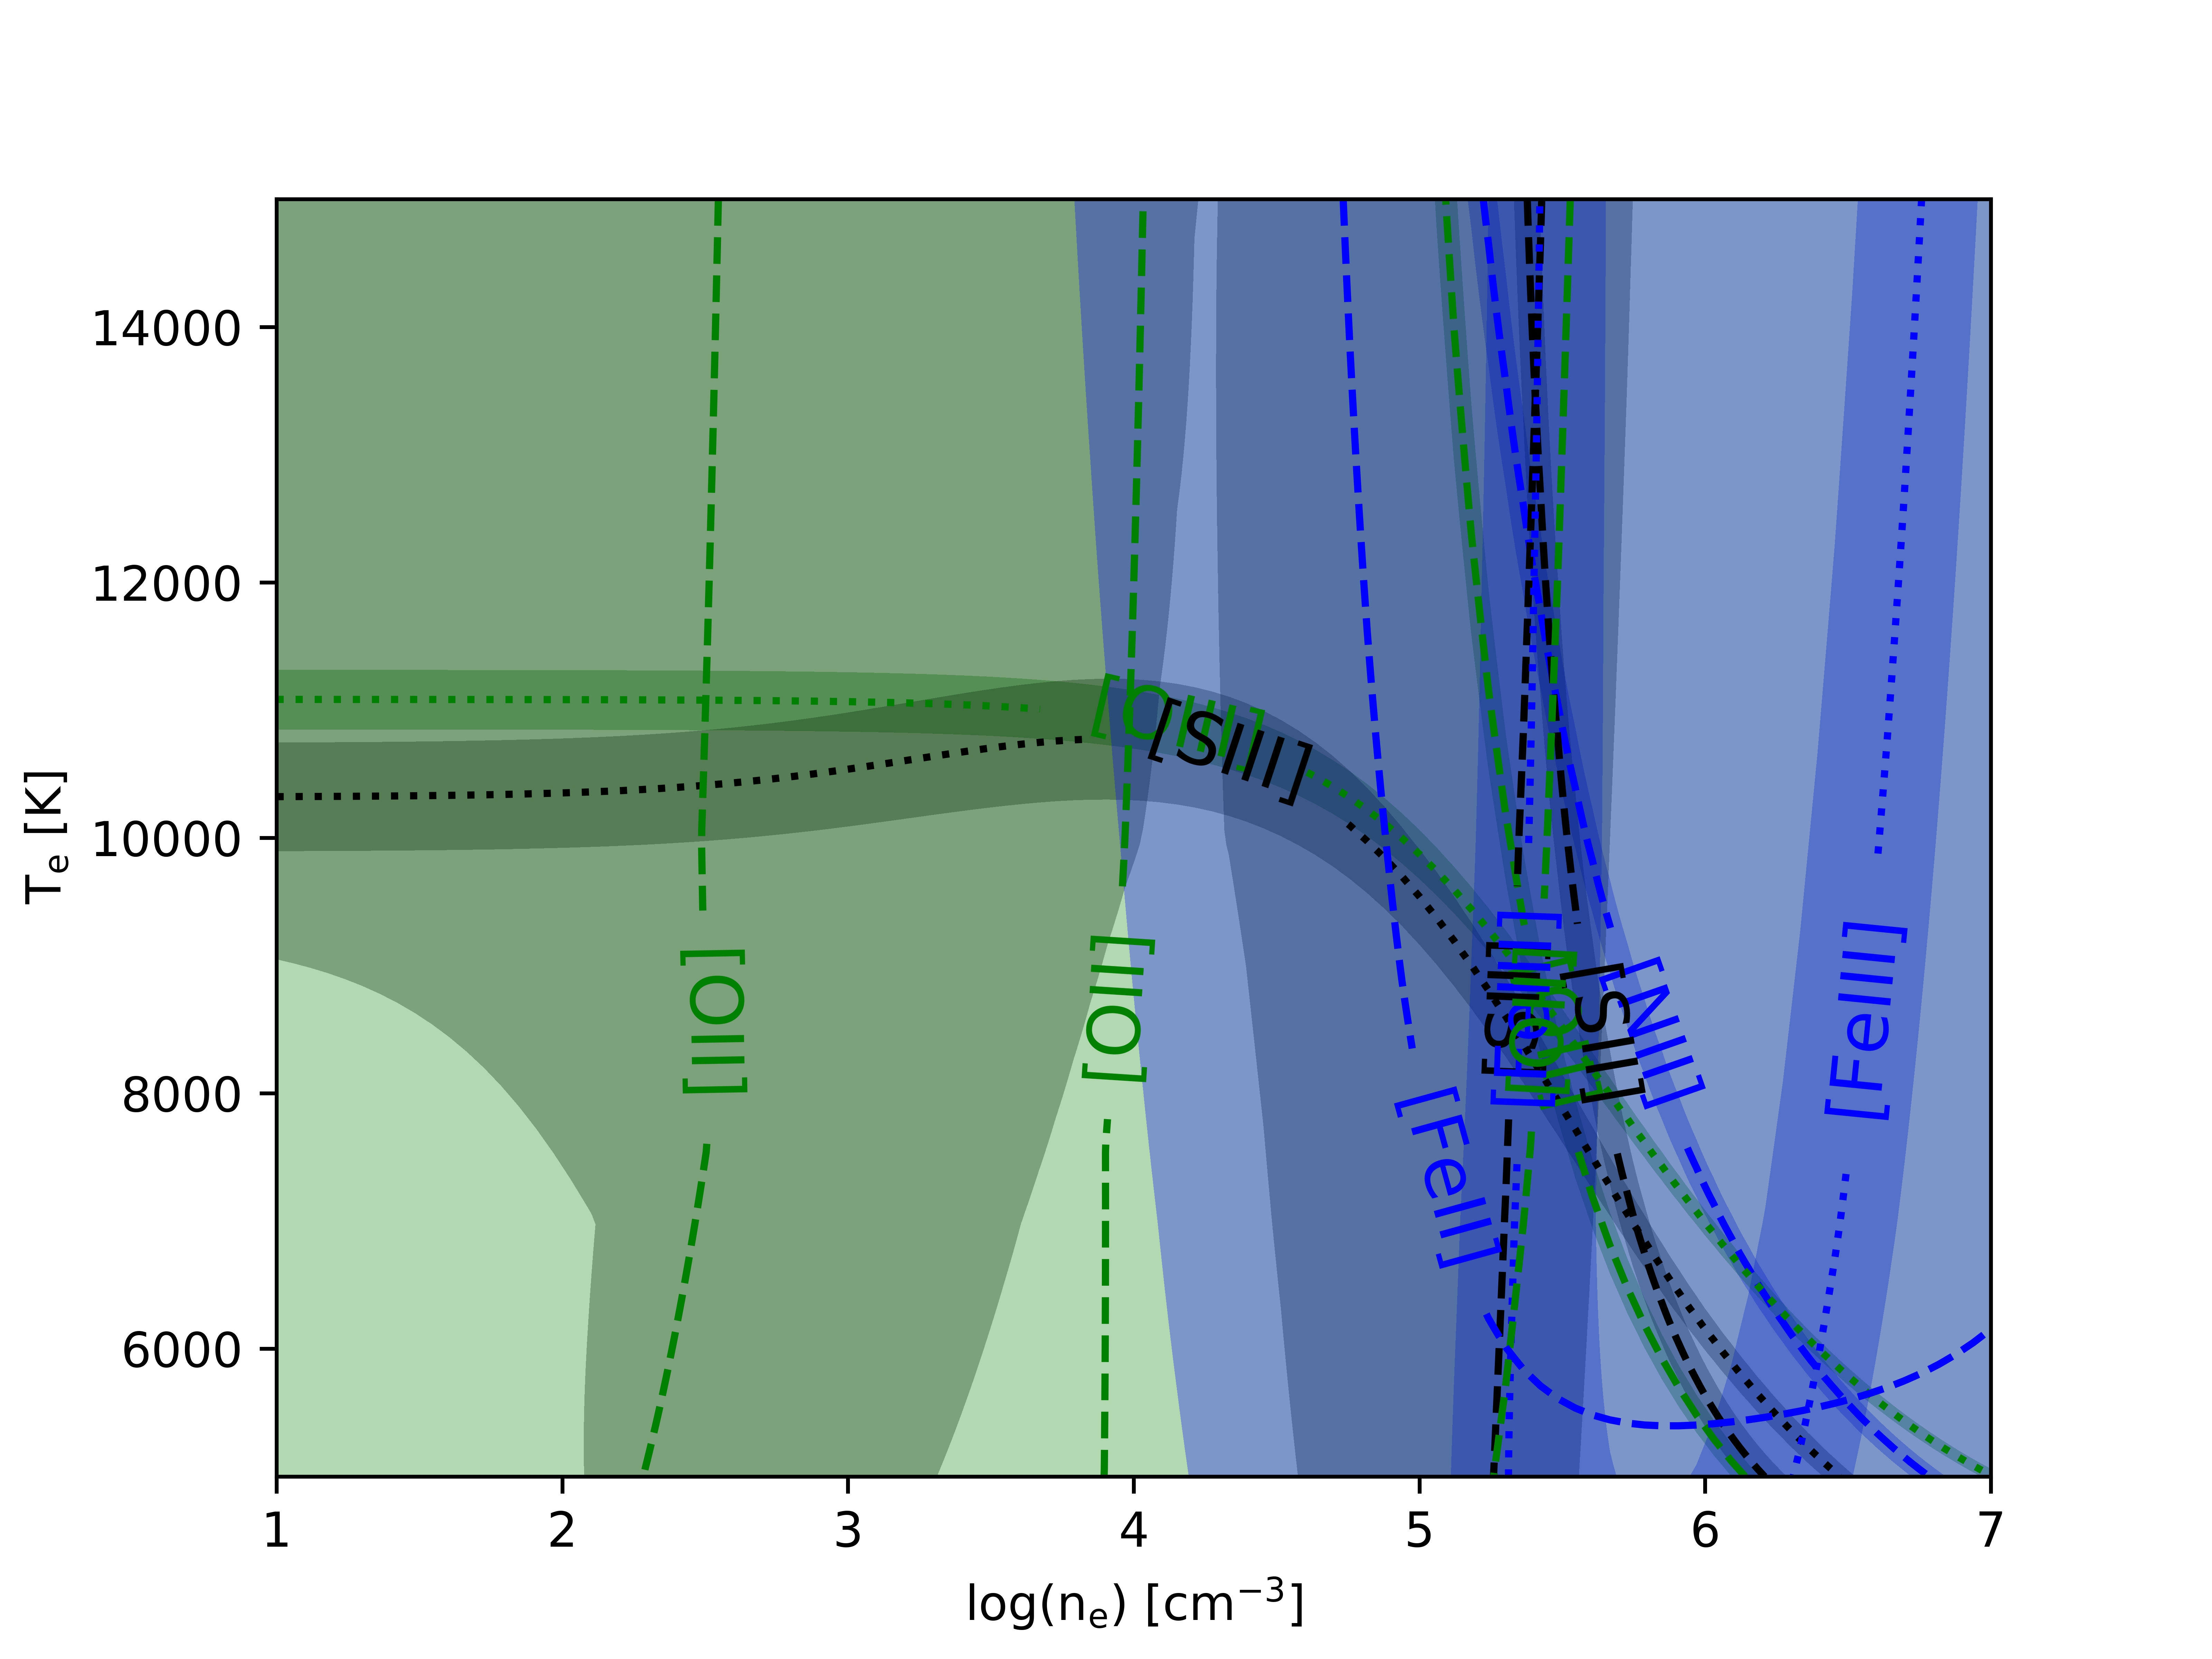
\includegraphics[height=4cm,width=\columnwidth]{HH514I.png}
    \caption{Cut~1, HH~514~I.}
  \end{subfigure}
  \begin{subfigure}{7.5cm}
     \centering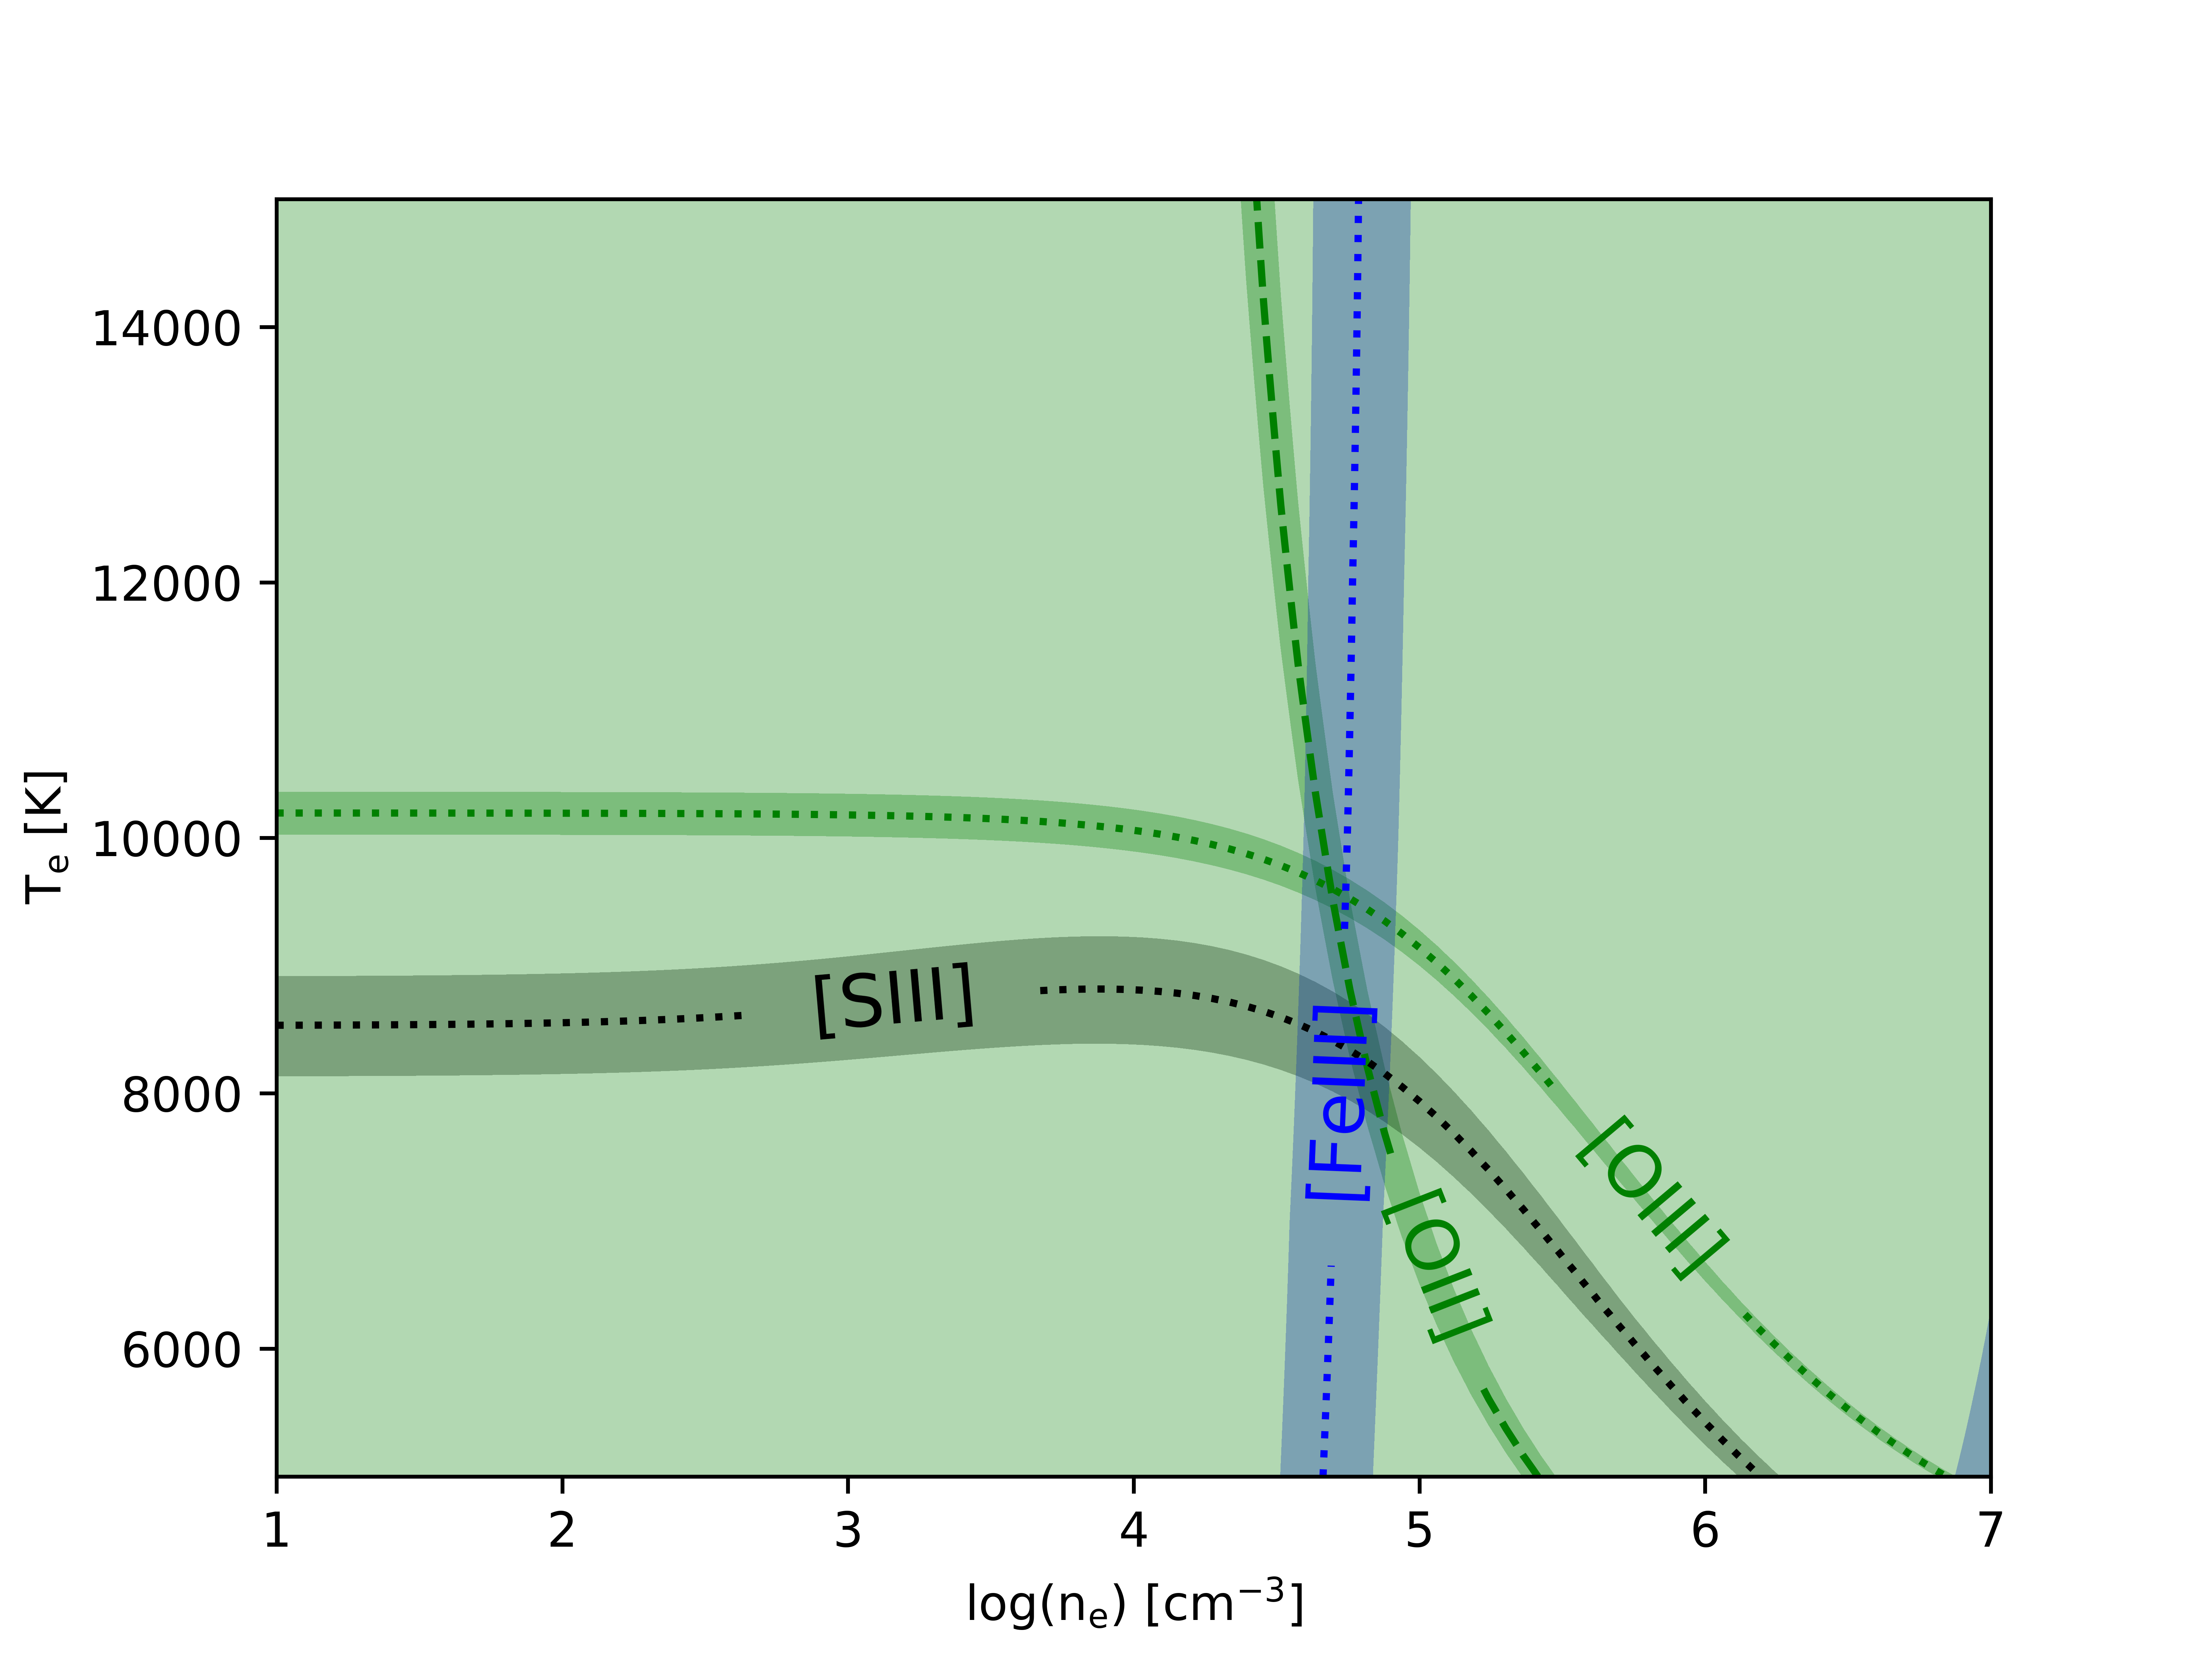
\includegraphics[height=4cm,width=\columnwidth]{HH514II.png}
    \caption{Cut~2, HH~514~II.}
  \end{subfigure}
 
  \begin{subfigure}{7.5cm}
   \centering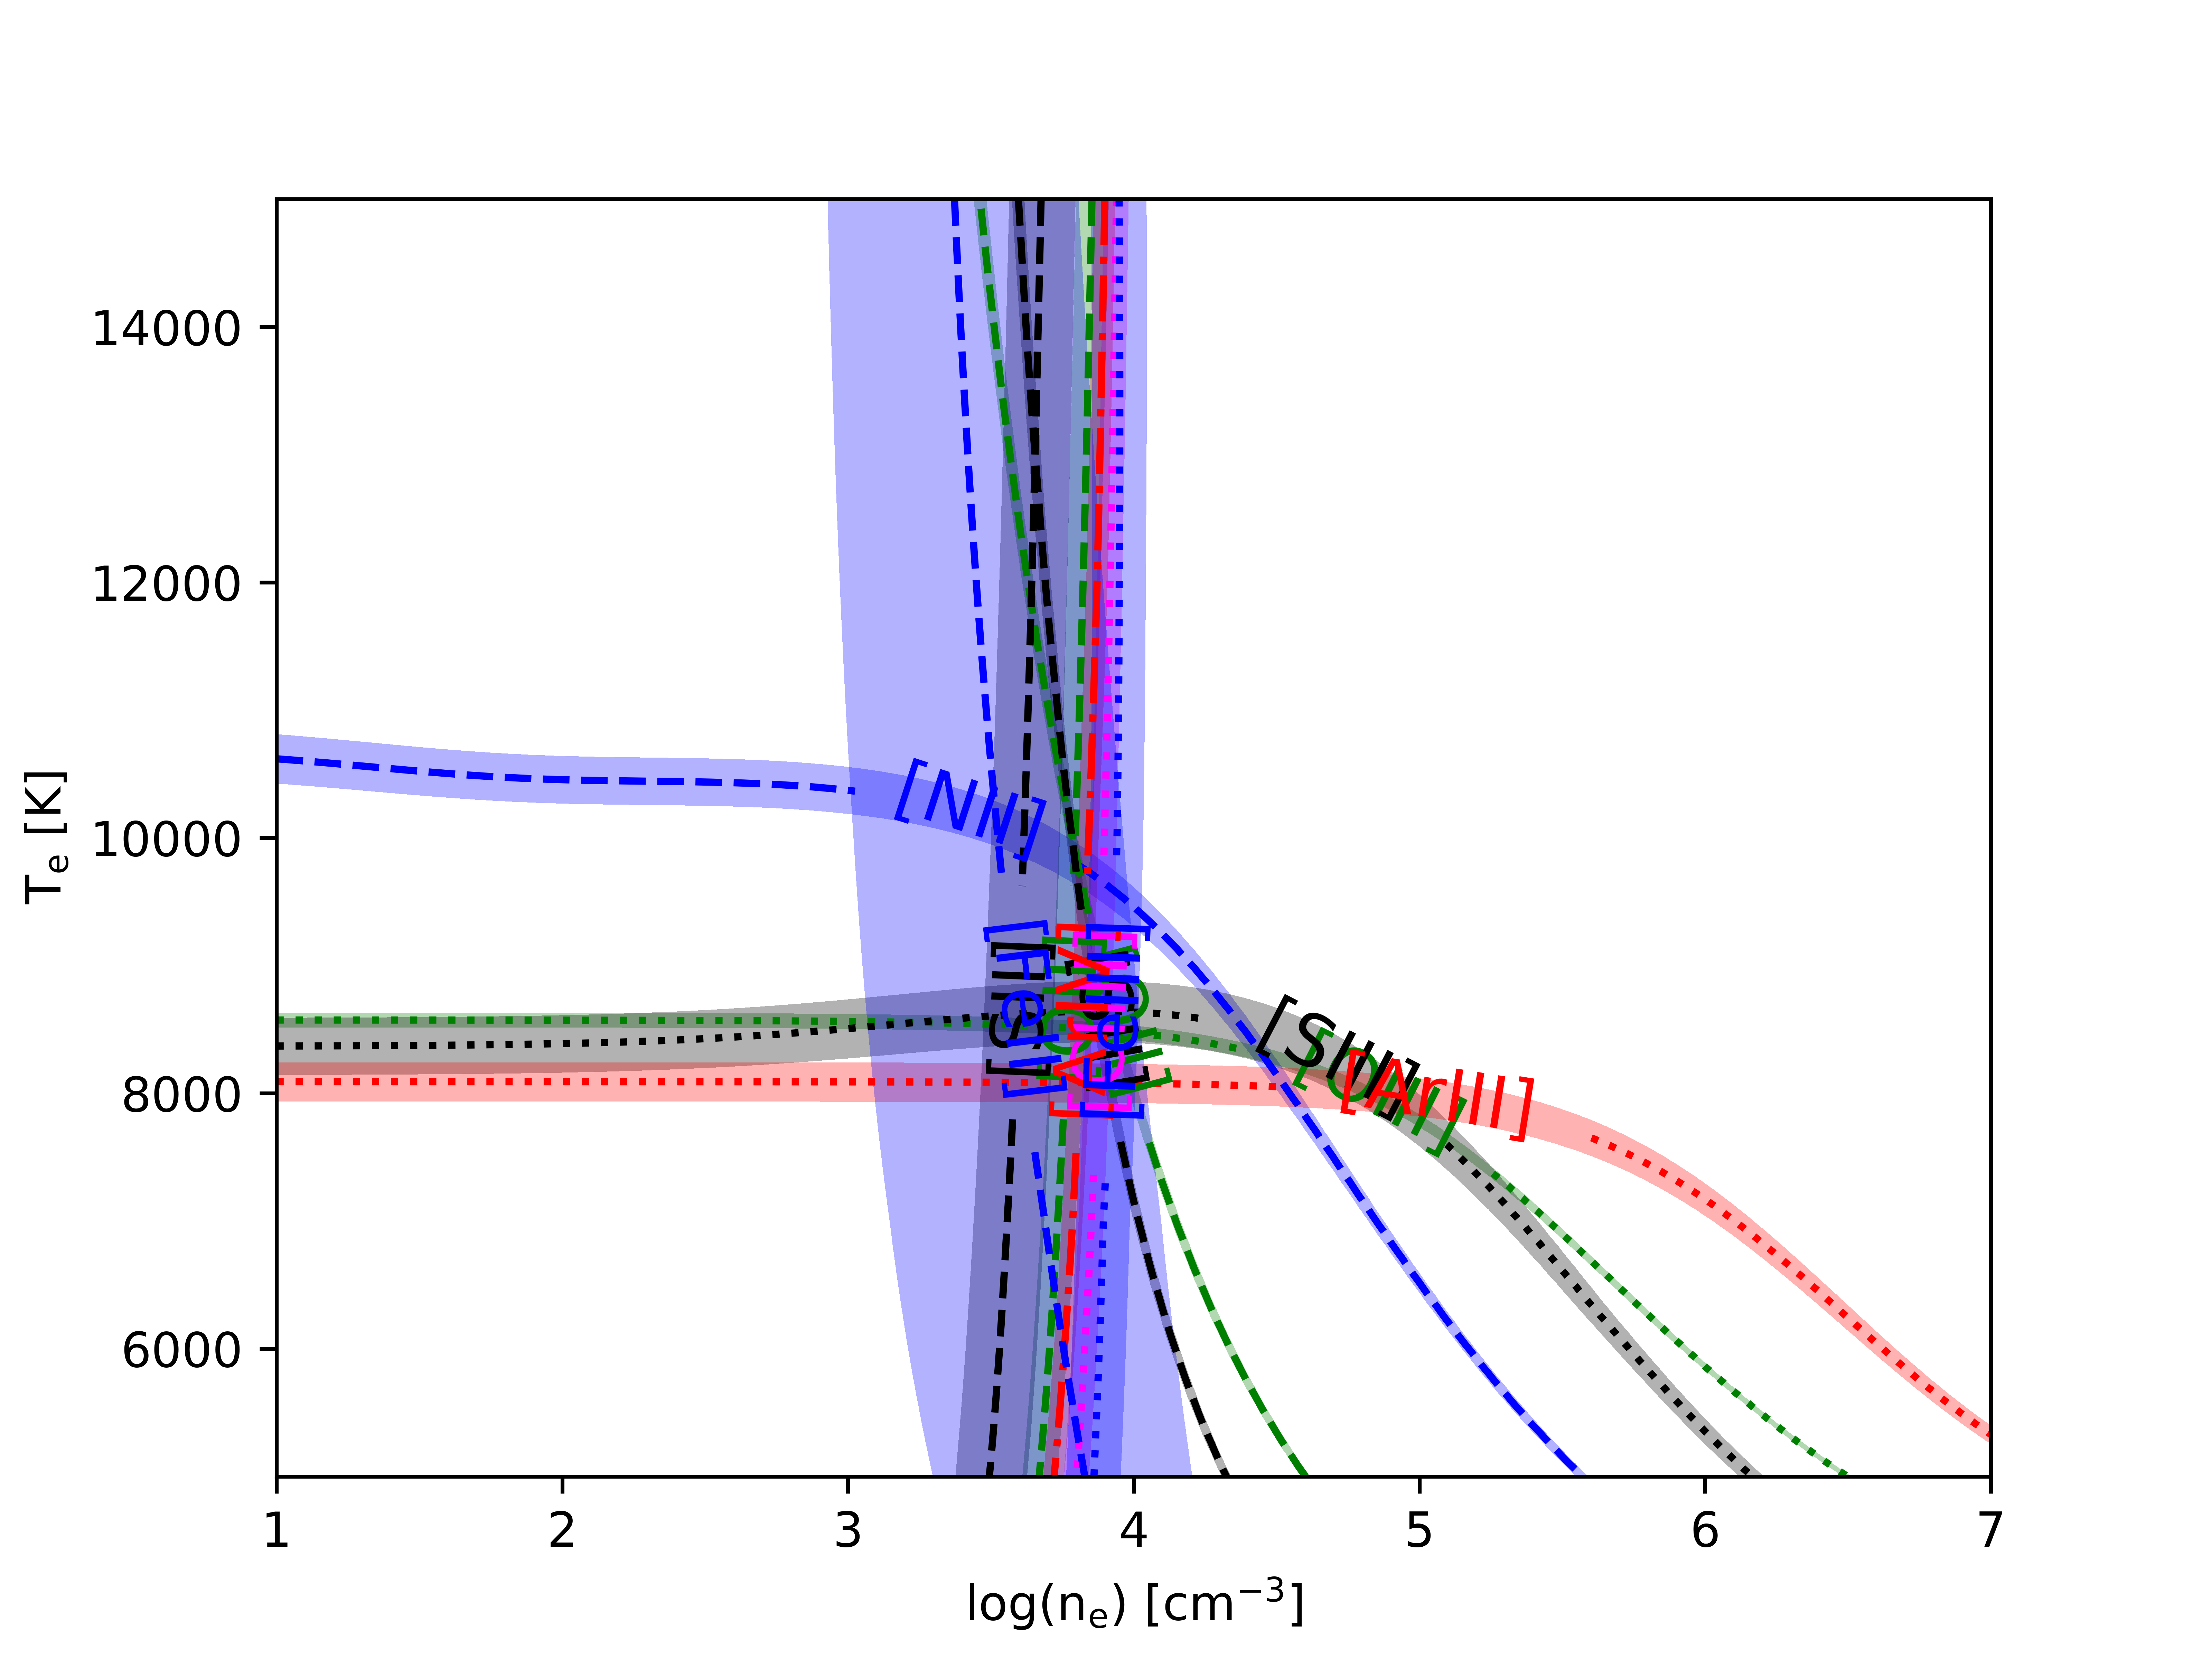
\includegraphics[height=4cm,width=\columnwidth]{neb_cut2.png}
   \caption{Cut~2, nebular component.}
  \end{subfigure}
  \begin{subfigure}{7.5cm}
    \centering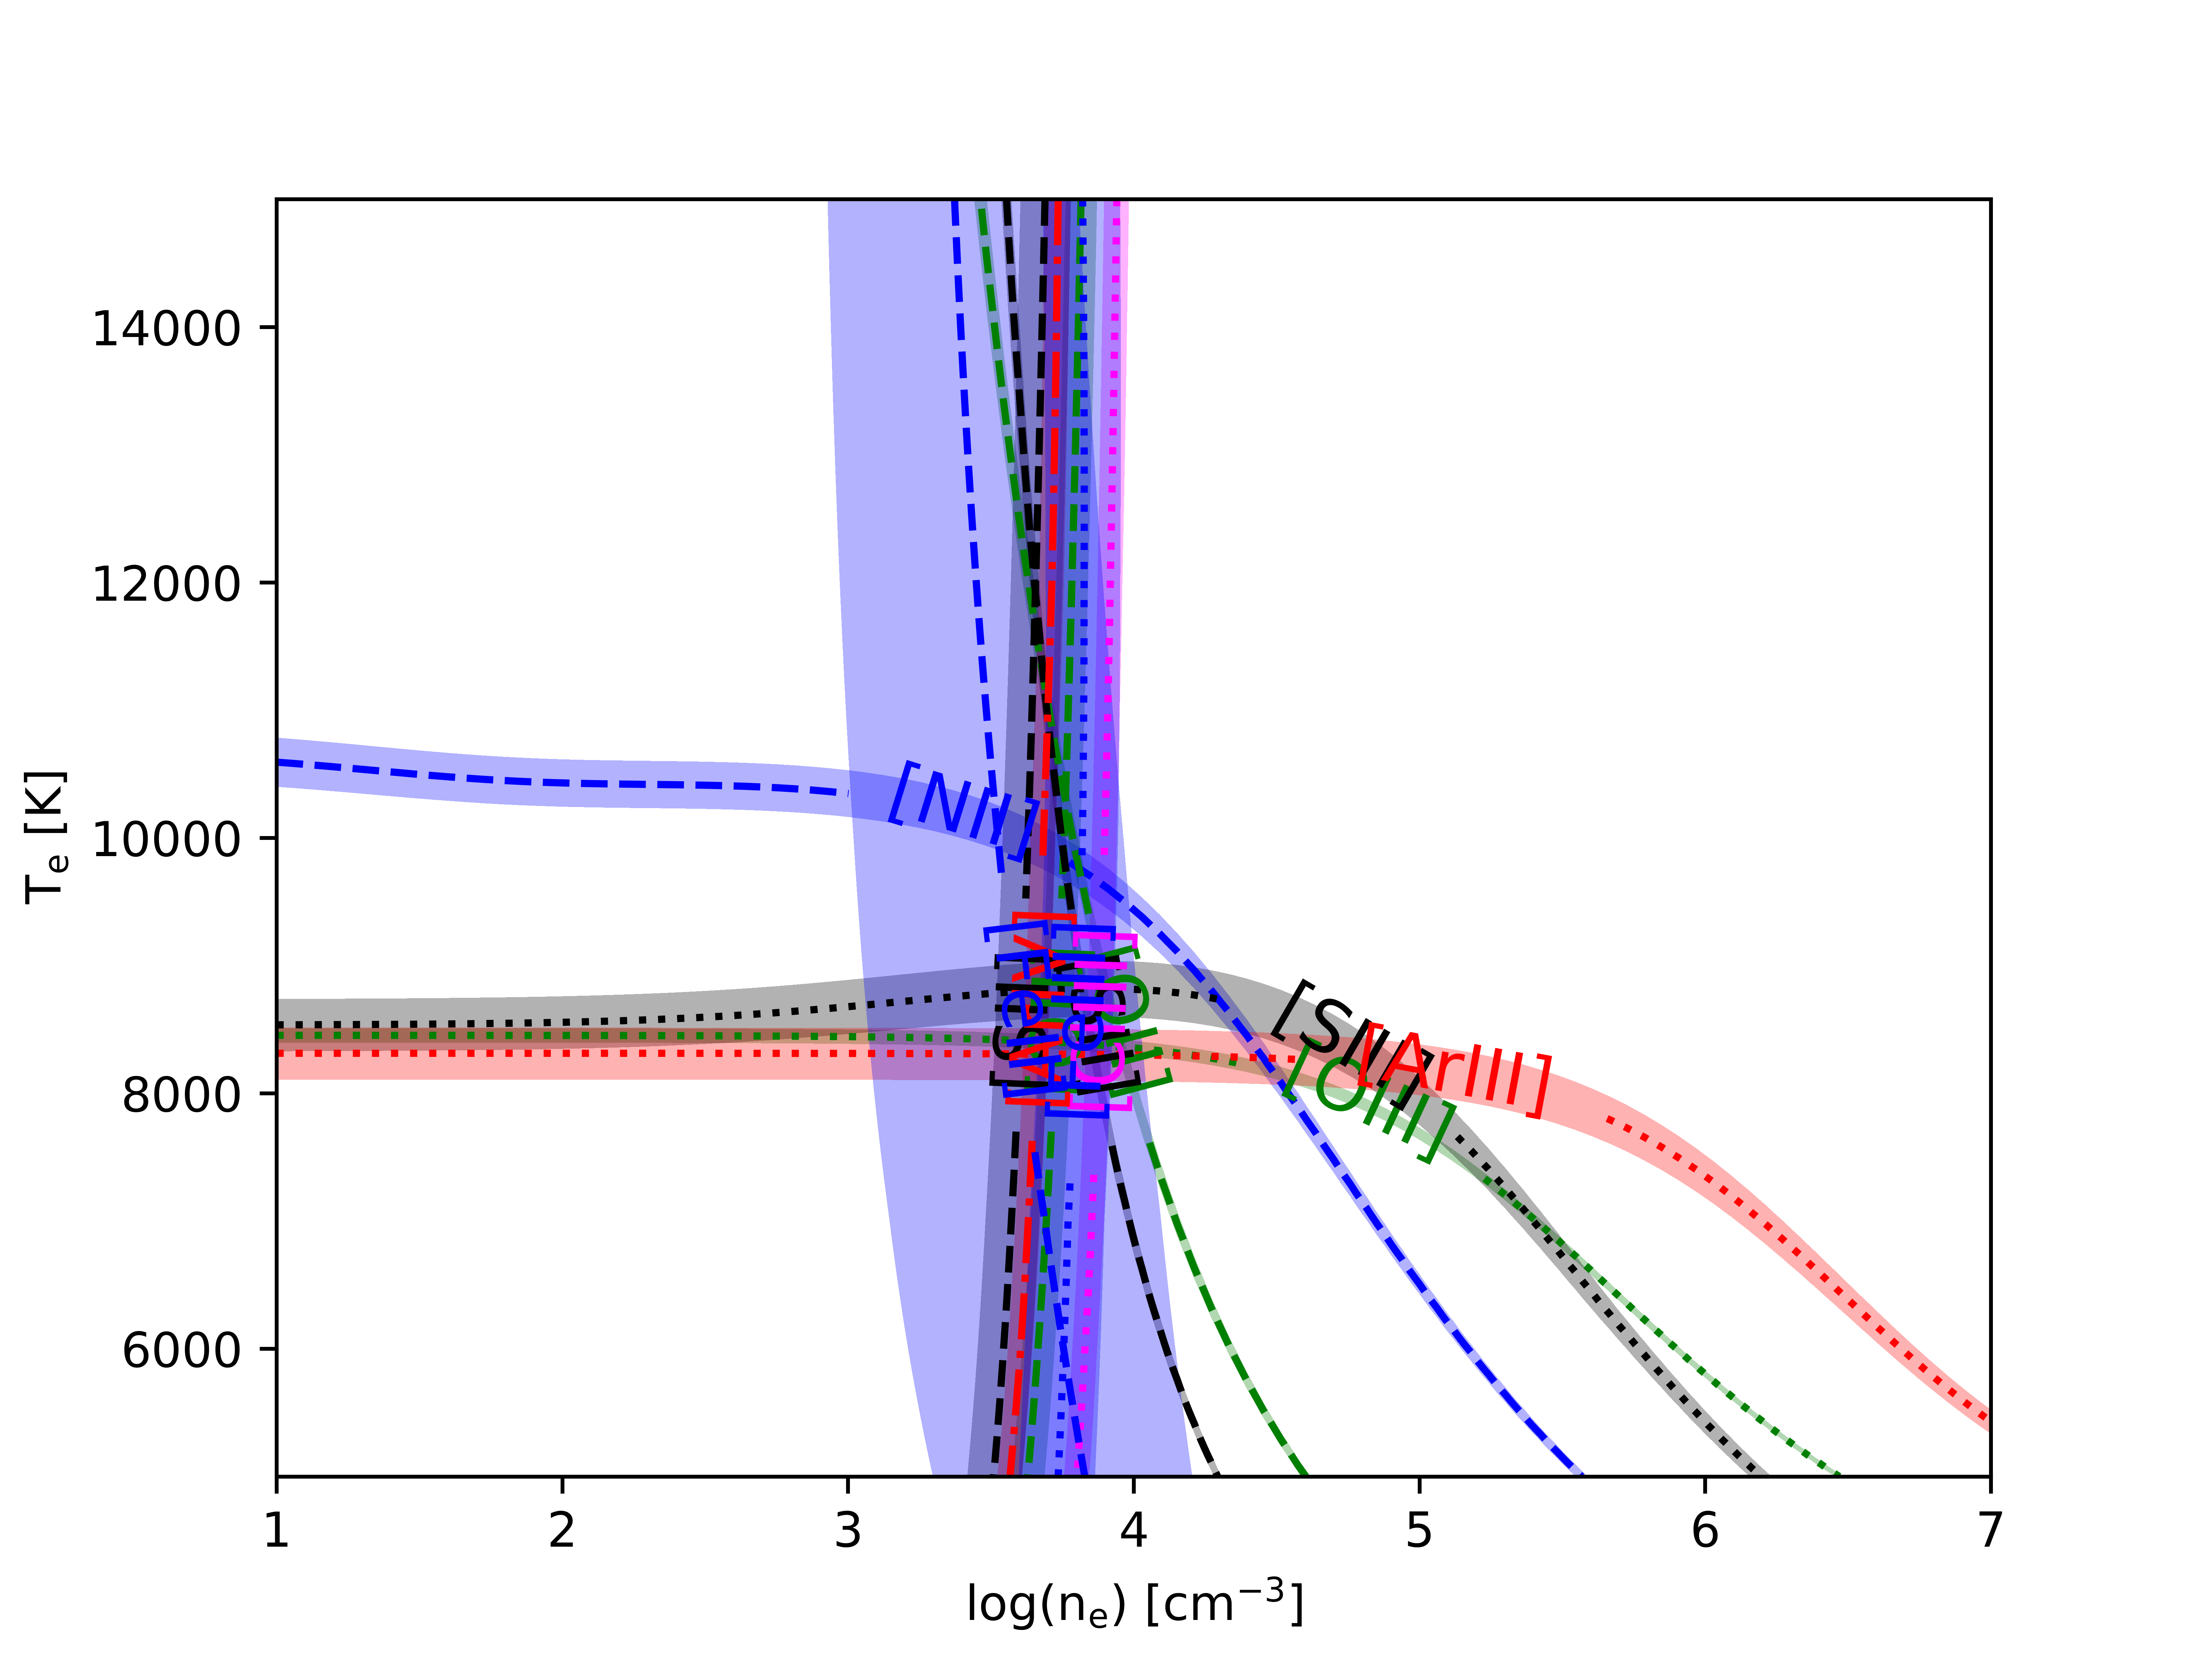
\includegraphics[height=4cm,width=\columnwidth]{neb_cut3.png}
    \caption{Cut~3, nebular component.}
  \end{subfigure}
  \caption{Plasma diagnostic plots for the individual analyzed components.}
\label{fig:plasma}
\end{figure*}




% Don't change these lines
\bsp	% typesetting comment
\label{lastpage}
\end{document}

% End of mnras_template.tex





\begin{table*}
\centering
\caption{}
\label{tab:}
\begin{adjustbox}{width=\textwidth}
\begin{tabular}{ccccc}
\hline

 & \multicolumn{4}{c}{Trans. Probabilities} \\
 
 \multirow{5}{*}{Coll. Strengths} \\ 
  & & Q96\&J00 & BBQ10 & NP96  \\
  
  
 &Z96& $T_{\rm e}=7900 \pm 640$, $n_{\rm e}=247470 \pm 10100$ & $T_{\rm e}=8740 \pm 610$, $n_{\rm e}=525250 \pm 20200$ & $T_{\rm e}=10960 \pm 1110$, $n_{\rm e}=535350 \pm 20200$ \\
  & Q96  & $T_{\rm e}=7630 \pm 510$, $n_{\rm e}=252530 \pm 10100$ & $T_{\rm e}=8640 \pm 510$, $n_{\rm e}=545460 \pm 20200$ & $T_{\rm e}=10560 \pm 1010$, $n_{\rm e}=545460 \pm 20200$ \\
   & BBQ10 & $T_{\rm e}=14600 \pm 400$, $n_{\rm e}=252530 \pm 10100$ & $T_{\rm e}=19750 \pm 1410$, $n_{\rm e}=676770 \pm 20200$ & $T_{\rm e}=19950 \pm 1410$, $n_{\rm e}=666670 \pm 30300$\\  
  & BB14 & $T_{\rm e}=7420 \pm 610$, $n_{\rm e}=444450 \pm 20200$ & $T_{\rm e}=10860 \pm 810$, $n_{\rm e}=929290 \pm 20200$& $T_{\rm e}=13480 \pm 1410$, $n_{\rm e}=989900 \pm 10100$\\
 
 
 \hline

\end{tabular}
\end{adjustbox}
\end{table*}



\begin{table*}
\centering
\caption{Comparison of the observed [Fe\thinspace III] intensity ratios and theoretical ones predicted by the transition probabilities adopted in Table~\ref{tab:atomic_data}}
\label{tab:fe3_ratios_theo}
\begin{adjustbox}{width=\textwidth}
\begin{tabular}{lcccccccccccc}
\hline
 & \multicolumn{1}{c}{Cut 1} & \multicolumn{2}{c}{Cut 2} & \multicolumn{1}{c}{Cut 3} & \\
Diagnostic &  HH514-I & Nebula & HH514-II  & Nebula & Prediction\\
\hline
4667/4734$^{a}$  & $0.36 \pm 0.02$ & $0.54 \pm 0.03$ & $0.54 \pm 0.04$ & $0.64 \pm 0.07$ & 0.28 & \\

4778/4734$^{b}$ & $0.63 \pm 0.04$ & $0.50 \pm 0.03$ & $0.80 \pm 0.06$ & $0.55 \pm 0.06$ & 0.48 & \\

4778/4667$^{a,b}$ & $1.79 \pm 0.14$ & $0.92 \pm 0.06$& $1.48 \pm 0.12$ & $0.85 \pm 0.12$ & 1.74 & \\

4607/4702$^{c,d}$ & $0.27 \pm 0.02$ & $0.31 \pm 0.01$ & $0.45 \pm 0.03$ & $0.28 \pm 0.02$ & 0.17 & \\
4607/4770$^{c}$ & $0.71 \pm 0.04$ & $0.86 \pm 0.05$ & $1.00 \pm 0.09$& $0.70 \pm 0.06$ & 0.51& \\

4702/4770$^{d}$  & $2.60 \pm 0.11$ & $2.81 \pm 0.13$ & $2.22 \pm 0.15$ & $2.53 \pm 0.17$ & 2.93 & \\

4658/4755$^{e}$  & $6.48 \pm 0.35$ & $5.24 \pm 0.19$ & $5.46 \pm 0.52$ & $4.85 \pm 0.22$ & 5.49 & \\
5011/5085 & - &$5.22 \pm 0.99$& - & - &5.94& \\
5271/5412 &  $10.51 \pm 1.77$ & $10.60 \pm 1.15$ & - & $11.14 \pm 1.76$ & 11.01 &\\
4881/4987$^{f}$  & $5.79 \pm 0.90$ & $4.97 \pm 0.29$ & $4.38 \pm 0.58$ & $5.48 \pm 0.86$ & 5.76 & \\
\hline
\end{tabular}
\end{adjustbox}
\begin{description}
\item $^a$ $\lambda$4667.11 affected by ghost in the nebular components. \\
\item $^b$ $\lambda$4777.70 in the high-velocity components is blended with the nebular component of N\thinspace II $\lambda$4779.72. \\
\item $^{c}$ [Fe\thinspace III] $\lambda 4607.12$ blended with  N\thinspace II $\lambda 4607.15$ in the nebular components while in the high-velocity ones is affected by a ghost feature.\\
\item $^{d}$ [Fe\thinspace III] $\lambda 4701.64$ was deblended from a ghost feature in the high-velocity components. \\
\item $^{e}$ [Fe\thinspace III] $\lambda 4754.81$ was deblended from a ghost feature in the high-velocity components. \\
\item $^{f}$ [Fe\thinspace III] $\lambda 4987.29$ blended with  N\thinspace II $\lambda 4987.38$ in the nebular components. \\
\end{description}
\end{table*}


